\documentclass[11pt]{article}

% Packages

% Basic math and fonts
\usepackage{amsmath, amsfonts, amssymb, mathtools}

% Encoding and language
\usepackage[T1]{fontenc}
\usepackage[italian]{babel}

% Layout and formatting
\usepackage[a4paper, margin=1in]{geometry}
\geometry{top=2cm, bottom=2cm, left=2.5cm, right=2.5cm}
\usepackage{caption}
\usepackage{float}
\usepackage{graphicx}
\usepackage{ragged2e}
\usepackage{multirow}

% Hyperlinks
\usepackage{url}
\usepackage{breakurl}
\usepackage{hyperref}
\hypersetup{
    colorlinks=true,
    linkcolor=black,
    urlcolor=blue,
    citecolor=black
}

% Plotting
\usepackage{pgfplots}
\pgfplotsset{compat=1.18}

% Header and footer
\usepackage{fancyhdr}
\setlength{\headheight}{14pt}
\pagestyle{fancy}
\fancyhf{}
\fancyhead[L]{\nouppercase{\leftmark}}
\fancyfoot[C]{\thepage}
\renewcommand{\sectionmark}[1]{\markboth{#1}{}}

\usepackage{attachfile2}

\usepackage{url}
\usepackage{breakurl}
\usepackage[backend=biber,style=numeric,url=true]{biblatex}
\addbibresource{../references.bib}
\DeclareFieldFormat{url}{\newline\url{#1}}
\setlength{\bibitemsep}{1em}


% DOCUMENT'S FIRST PAGE ---------------------------------------------------------------------------------------------------------------------
\begin{document}
\thispagestyle{empty}

\begin{flushright}
    
\includegraphics[width=0.4\linewidth]{images/Politecnico di Torino logo.pdf}
\end{flushright}

\vspace*{7cm}

\begin{flushleft}
    {\Huge\bfseries Impianto industriale} \\
    \vspace{1em}
    {\large A.A. 2024-2025} \\
    \vspace{4em}

    {\Large\bfseries Gruppo 1} \\
    \vspace{1em}
    \begin{tabular}{ll|ll}
        \multicolumn{2}{c|}{\textbf{Team A}} & \multicolumn{2}{c}{\textbf{Team B}} \\
        \large {{studentName0}} & \large {{studentId0}} & \large {{studentName8}} & \large {{studentId8}} \\
        \large {{studentName1}} & \large {{studentId1}} & \large {{studentName9}} & \large {{studentId9}} \\
        \large {{studentName2}} & \large {{studentId2}} & \large {{studentName10}} & \large {{studentId10}} \\
        \large {{studentName3}} & \large {{studentId3}} & \large {{studentName11}} & \large {{studentId11}} \\
        \large {{studentName4}} & \large {{studentId4}} & \large {{studentName12}} & \large {{studentId12}} \\
        \large {{studentName5}} & \large {{studentId5}} & \large {{studentName13}} & \large {{studentId13}} \\
        \large {{studentName6}} & \large {{studentId6}} & \large {{studentName14}} & \large {{studentId14}} \\
        \large {{studentName7}} & \large {{studentId7}} & \large {{studentName15}} & \large {{studentId15}} \\
    \end{tabular}

\end{flushleft}

\vfill

% TABLE OF CONTENTS ---------------------------------------------------------------------------------------------------------------------
\newpage
\thispagestyle{empty}
\tableofcontents

% LIST OF FIGURES ----------------------------------------------------------------------------------------------------------------------
\newpage
\thispagestyle{empty}
\listoffigures

% LIST OF ABBREVIATIONS -----------------------------------------------------------------------------------------------------------------
\newpage
\thispagestyle{empty}
\section*{Lista delle abbreviazioni}
\begin{itemize}
    \item UdC: Unità di carico
    \item OEE: Overall Equipment Effectiveness
    \item WBS: Work Breakdown Structure
    \item OBS: Organizational Breakdown Structure
    \item VSM: Value Stream Mapping
    \item HR: Human Resources
    \item TC: Tempo ciclo
    \item TT: Takt Time
    \item A: Availability (disponibilità)
    \item UE: Uptime Efficiency (performance)
    \item QR: Quality Rate (tasso di qualità)
    \item SAT: Saturazione
    \item RPW: Ranking Position Weight
    \item NIOSH: National Institute for Occupational Safety and Health
    \item EPEI: Every Part Every Interval
    \item ODETTE: Organization for Data Exchange by Tele Transmission in Europe
    \item $\text{Int}_R$: intervallo di riordino
    \item IR: indice di rotazione
    \item MP: Materie Prime
    \item PF: Prodotti Finiti
\end{itemize}
\newpage

% START -----------------------------------------------------------------------------------------------------------------
\section{Calcolo dei fabbisogni}
\subsection{Calcolo dei volumi}
Per il calcolo dei volumi di materiali in ingresso e uscita, sono stati considerati i seguenti dati:
\begin{itemize}
    \item Coefficiente di impiego
    \item Domanda mensile
    \item Quantità lorda
    \item QR per ciascuna operazione (saldatura e assemblaggio)
\end{itemize}

In prima battuta, sono state definite le quantità lorde dell'elemento assemblato finale (ovvero le due plance) ricavandone il valore dalle specifiche del progetto. Successivamente, sono state calcolate le quantità nette per ciascun componente, tenendo conto del coefficiente di impiego e della domanda mensile del componente "padre". Infine, è stato possibile calcolare le quantità lorde per ciascun componente, dividendo la quantità netta per il QR dell'operazione di riferimento.
\begin{equation}
    Q_\text{netta} = Q_\text{lorda,P} \times \text{coeff}_\text{impiego}
\end{equation}

\begin{equation}
    Q_\text{lorda} = \frac{Q_\text{netta}}{\text{QR}}
\end{equation}

L'operazione successiva è stata quella di definire il numero di pezzi che compongono i lotti dei due reparti di saldatura e assemblaggio per ciascun prodotto, andando a ricavare dalle specifiche del progetto il numero di lotti mensili.
\begin{equation}
    Q_\text{lotto} = \frac{Q_\text{lorda}}{N_\text{lotti mensili}}
\end{equation}

Di seguito, è possibile vedere un esempio di calcolo dei volumi di materiali in ingresso e uscita per il prodotto "(Corpo + Inserto) Plancia segmento A1" nella figura \ref{fig: Volumi materiale in ingresso e uscita}:
\begin{align*}
    & Q_\text{netta} = 25\,582 \cdot 1 = 25\,582 \\
    & Q_\text{lorda} = \frac{25\,582}{0,98} = 26\,104 \\
    & Q_\text{lotto} = \frac{26\,104}{4} = 6\,526
\end{align*}

\begin{figure}[H]
    \centering
    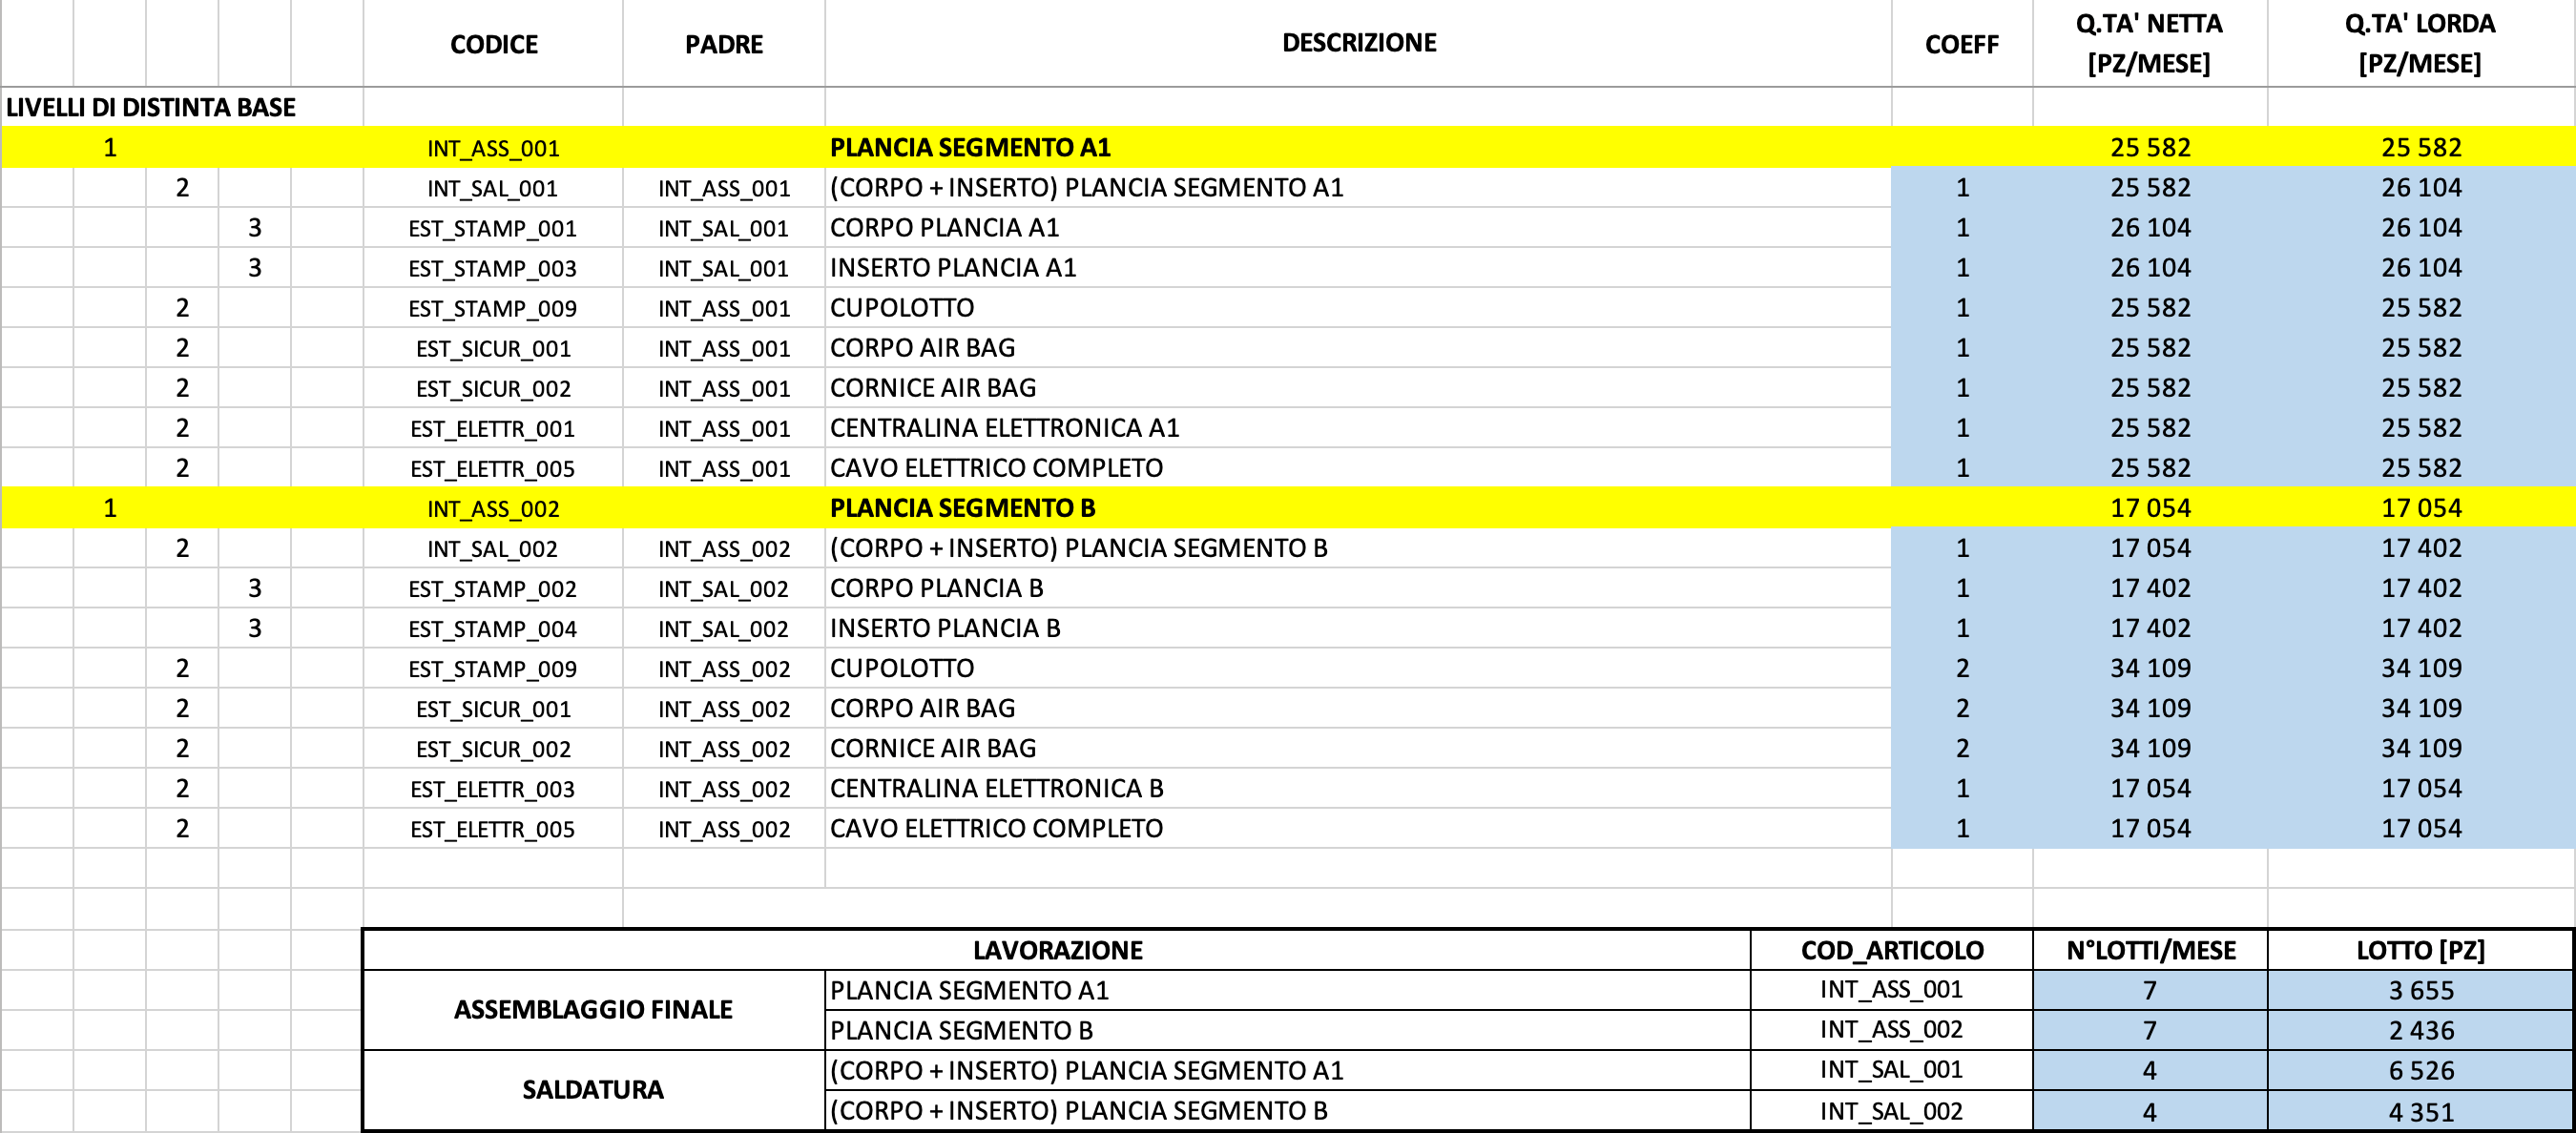
\includegraphics[width=\textwidth]{images/Volumi materiale in ingresso e uscita.png}
    \caption{Volumi materiale in ingresso e uscita}
    \label{fig: Volumi materiale in ingresso e uscita}
\end{figure}

\noindent
Tutti i calcoli sono disponibili negli allegati "{{excelA1B}}" e "{{excelA2D}}".
\newpage


\section{Ciclo di assemblaggio}
\subsection{Distinta base}
La distinta base ad albero rappresenta l'elenco dei materiali e dei componenti utilizzati accompagnati da un coefficiente di impiego.
In questo caso, sono state realizzate due distinte, una per ciascun processo produttivo (saldatura e assemblaggio).

Di seguito, è riportata la distinta base di un singolo prodotto alla luce del fatto che la loro costruzione segue la stessa logica:
\begin{figure} [H]
    \centering
    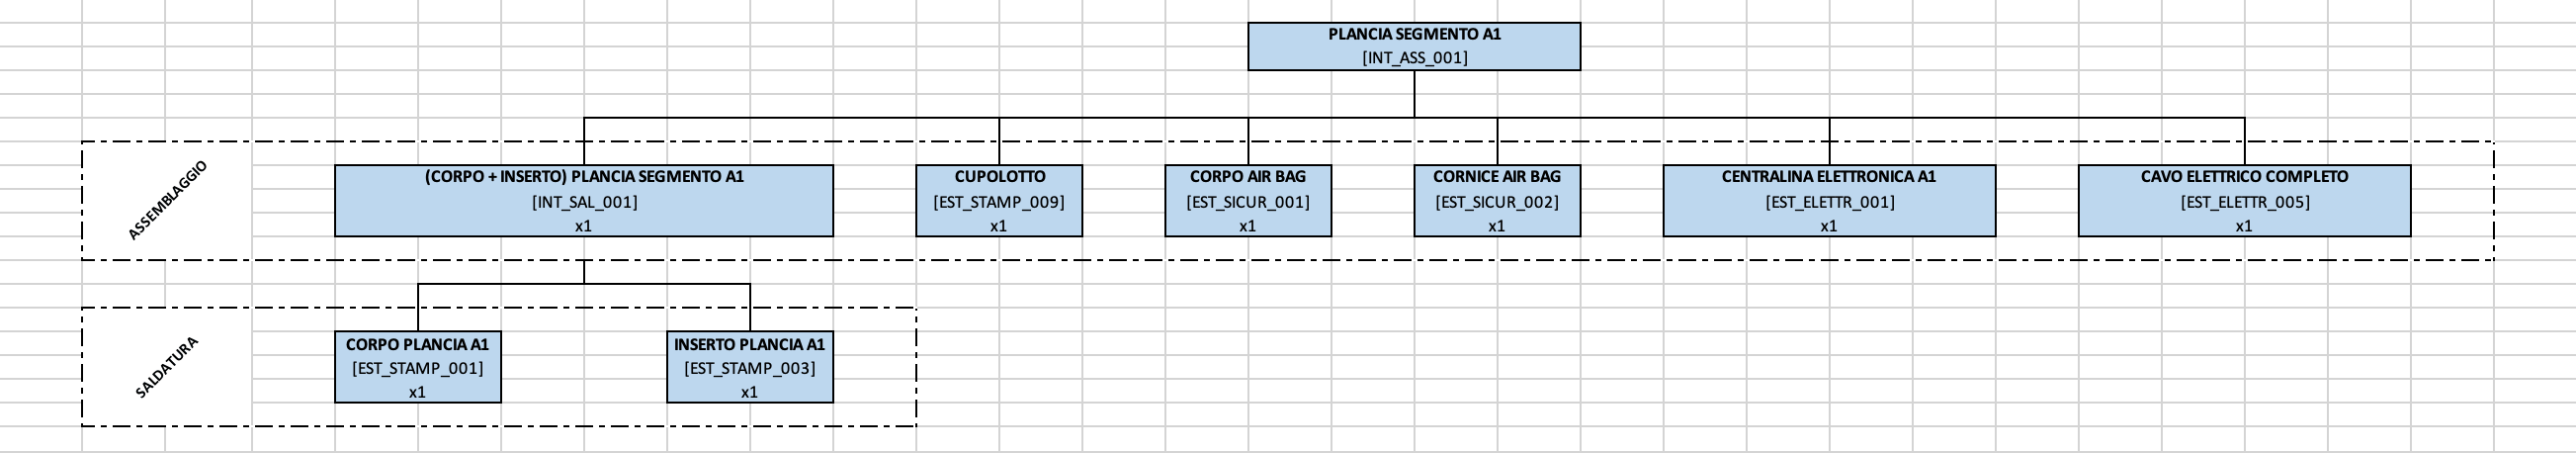
\includegraphics[width=\textwidth]{images/Distinta base A1.png}
    \caption{Distinta base ad albero A1}
    \label{fig: Distinta base ad albero A1}
\end{figure}

Le altre distinte base sono disponibili nell'allegato "{{distintaBase}}".
\vskip4em

\subsection{Diagramma di flusso}
Diversamente, il diagramma ad albero del processo produttivo si costruisce a partire dalla distinta base, andando ad invertire i collegamenti con i blocchi (quindi inserendo all'interno dei blocchi e le operazioni da eseguire e sui collegamenti, le materie prime, i semilavorati, …).

Come per la distinta base, anche in questo caso è riportato un solo esempio di processo produttivo:
\begin{figure} [H]
    \centering
    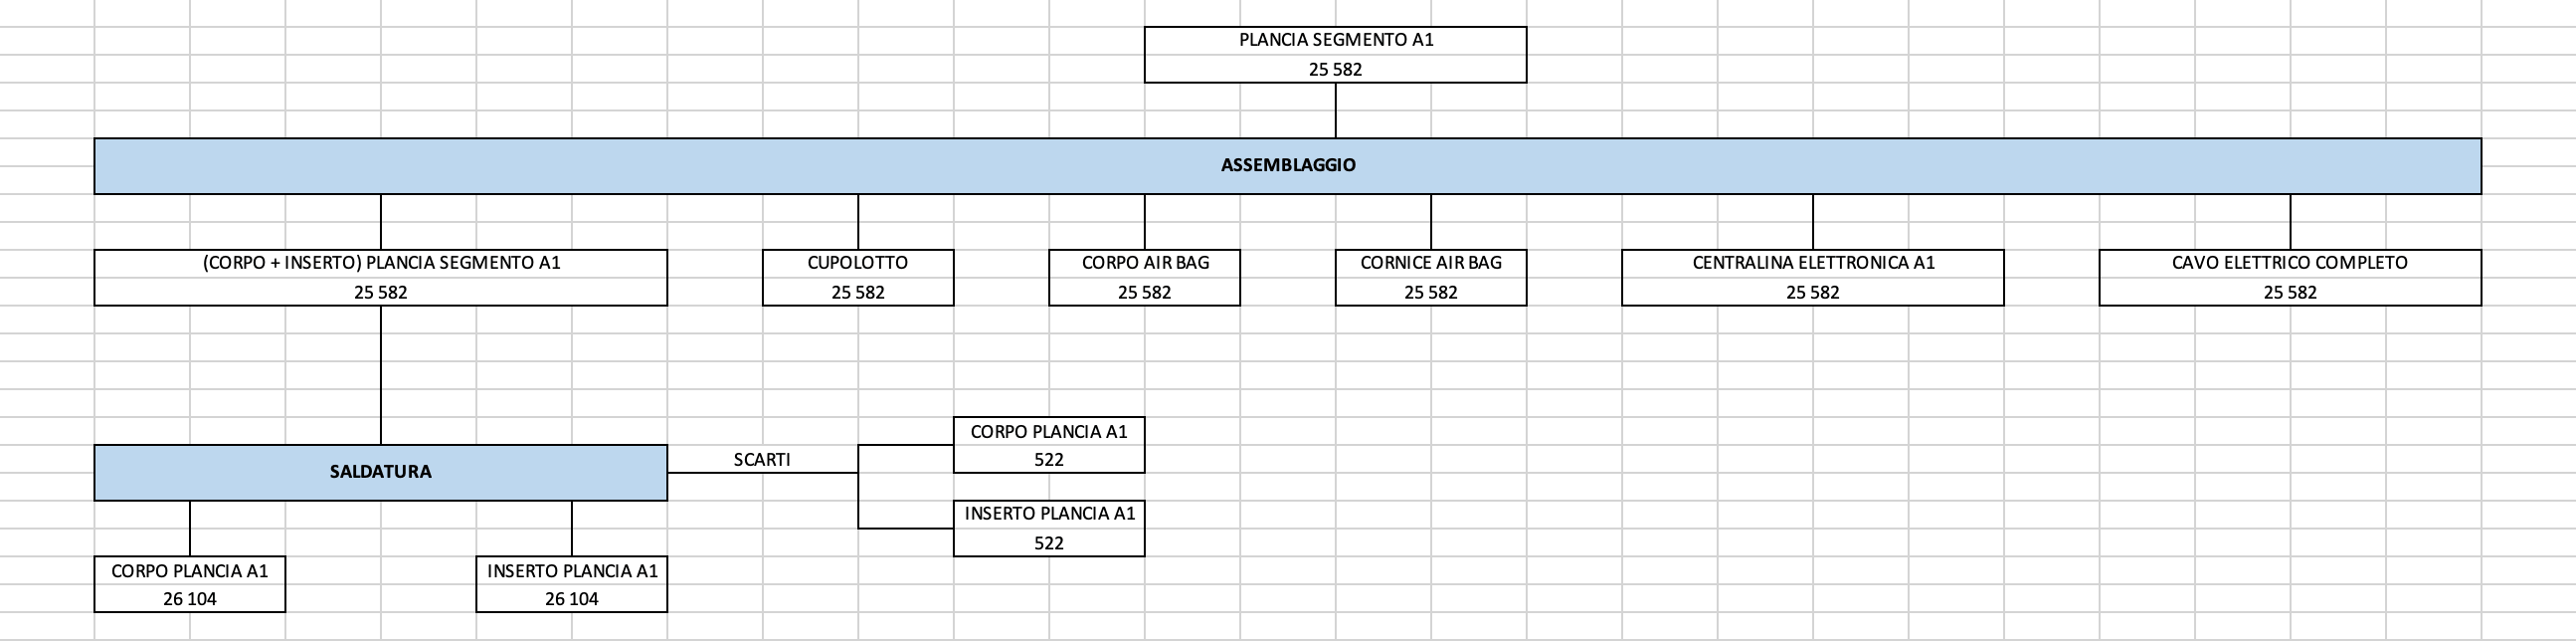
\includegraphics[width=\textwidth]{images/Processo produttivo A1.png}
    \caption{Processo produttivo A1}
    \label{fig: Processo produttivo A1}
\end{figure}

\noindent
Gli altri diagrammi ad albero sono disponibili nell'allegato "{{processoProduttivo}}".
\newpage

\subsection{Calcolo delle postazioni per assemblaggio [metodo RPW]}
Per il calcolo delle postazioni di assemblaggio, è stato definito il grafo delle operazioni di assemblaggio, che rappresenta le operazioni da eseguire e i collegamenti tra di esse.
\begin{figure} [H]
    \centering
    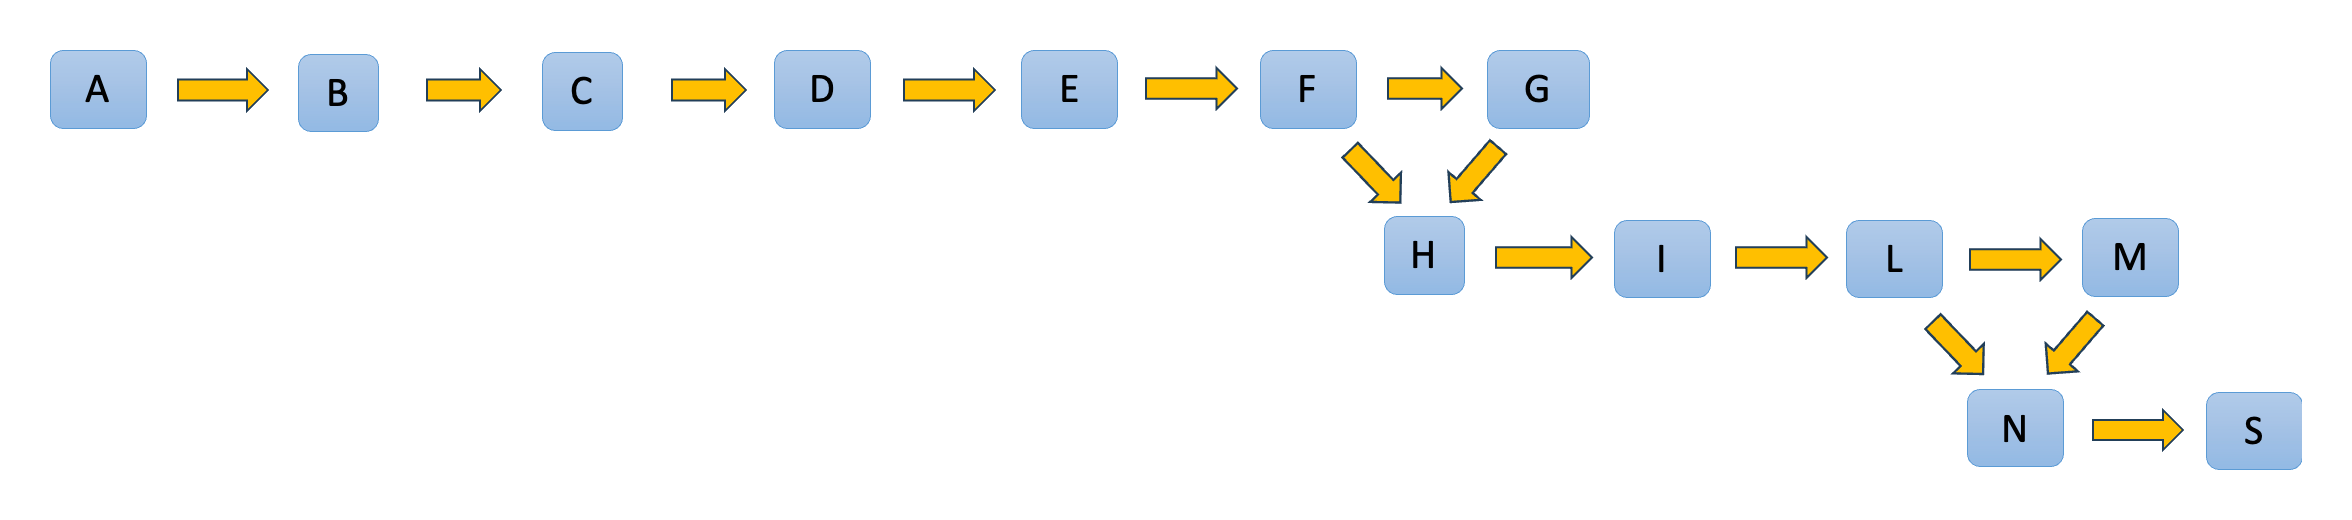
\includegraphics[width=\textwidth]{images/Grafo operazioni assemblaggio A1.png}
    \caption{Grafo delle operazioni di assemblaggio A1}
    \label{fig: Grafo delle operazioni di assemblaggio A1}
\end{figure}

Successivamente, è stato calcolato il tempo di assemblaggio per ciascuna operazione e il RPW per ciascuna operazione, che rappresenta il tempo di esecuzione dell'operazione più il tempo di esecuzione delle operazioni che la seguono.
\begin{equation}
    \text{RPW}_j = T_j + \sum_{i=1}^{n} T_i
\end{equation}

Grazie a questo, è possibile ottenere una tabella ordinata della varie operazioni di assemblaggio, come la seguente:
\begin{figure} [H]
    \centering
    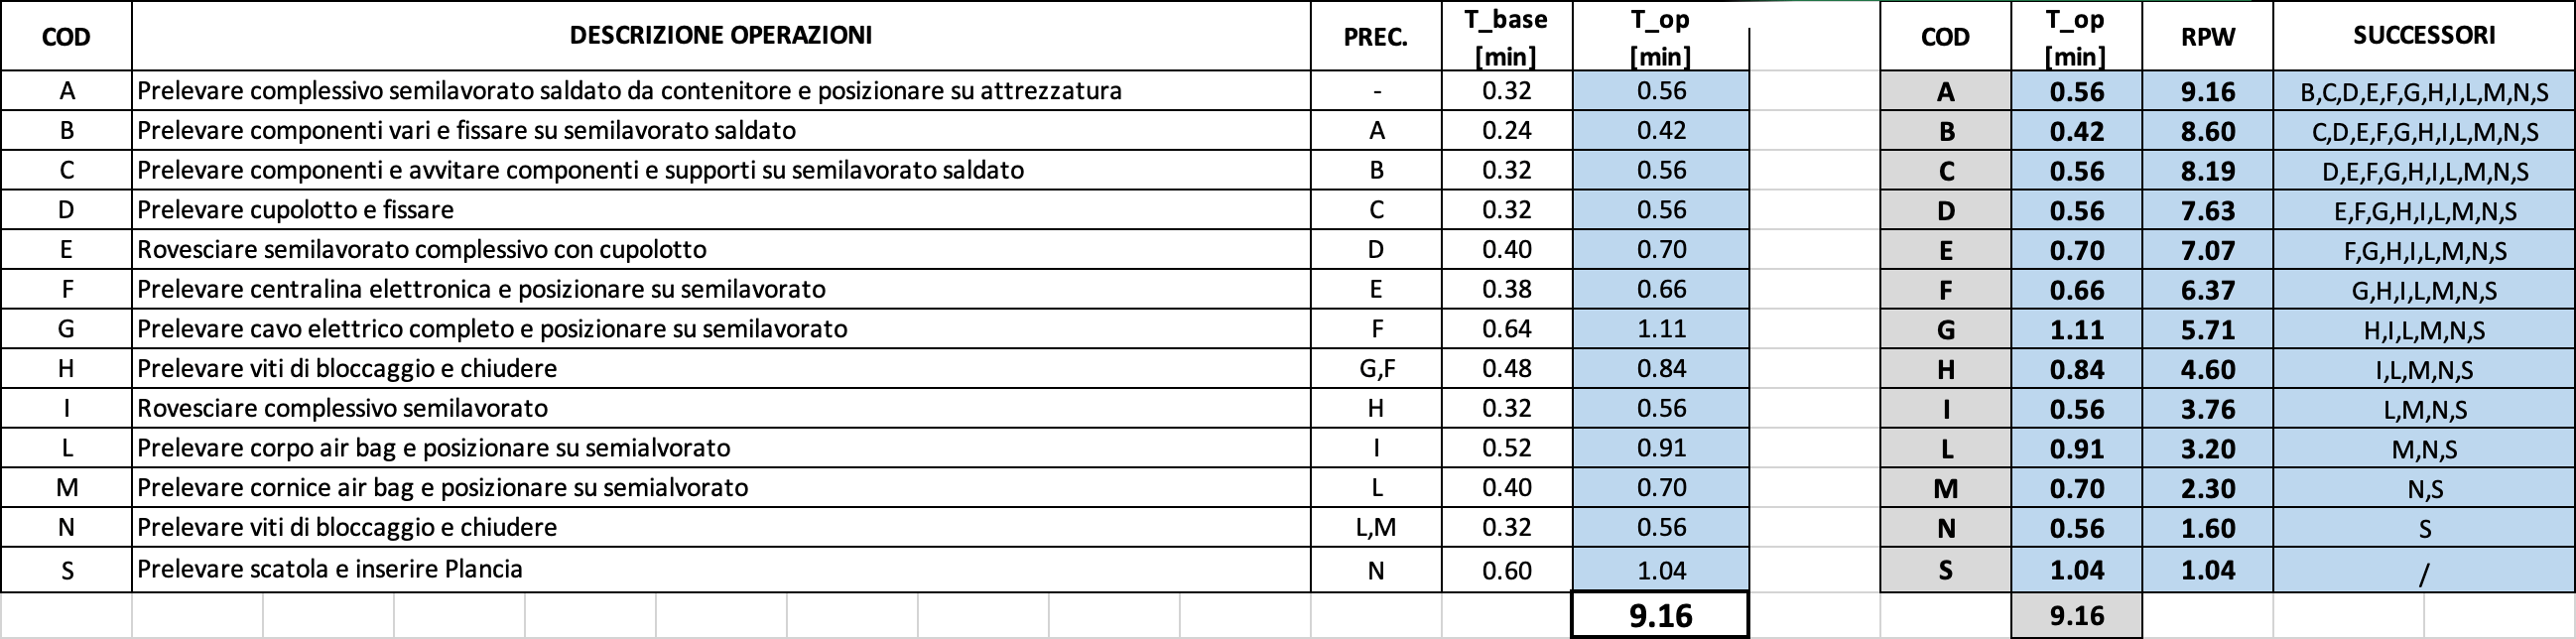
\includegraphics[width=\textwidth]{images/Tabella operazioni assemblaggio A1.png}
    \caption{Tabella delle operazioni di assemblaggio A1}
    \label{fig: Tabella delle operazioni di assemblaggio A1}
\end{figure}

Come ultimo passo, sono state raggruppate nella stessa postazione le operazione la cui somma dei tempi di esecuzione è minore di TC, ottenendo così il numero di postazioni di assemblaggio necessarie per ciascun prodotto.
\begin{figure} [H]
    \centering
    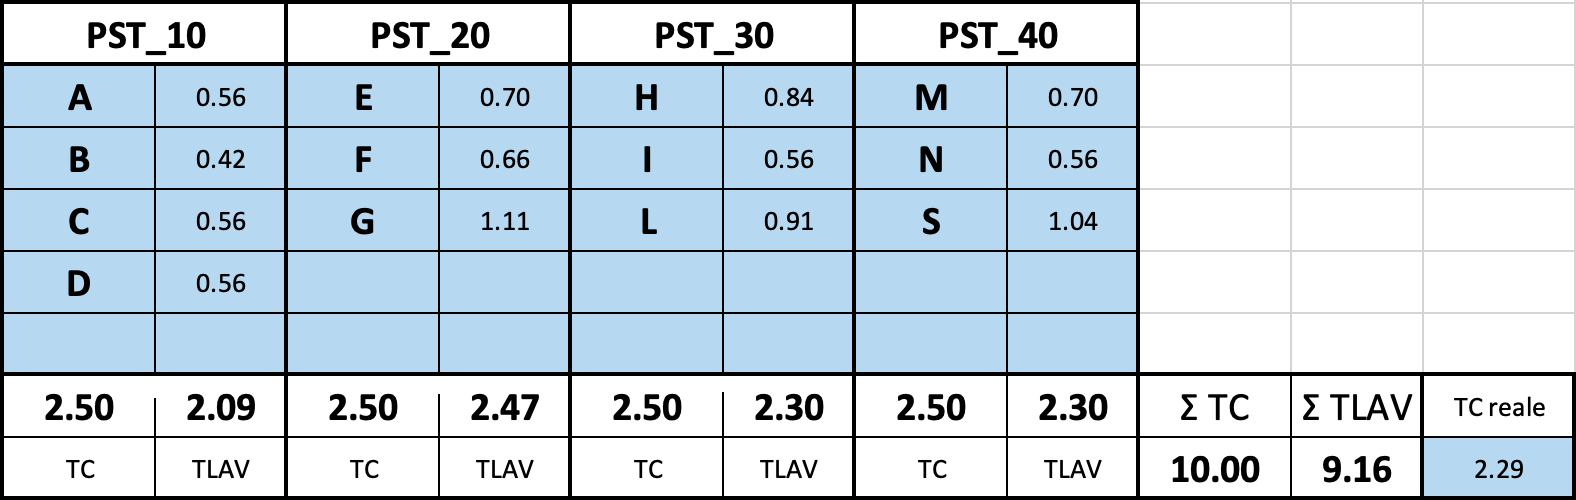
\includegraphics[width=\textwidth]{images/Postazioni assemblaggio A1.png}
    \caption{Postazioni di assemblaggio A1}
    \label{fig: Postazioni di assemblaggio A1}
\end{figure}

\newpage


\section{Processo produttivo}
\subsection{Calcolo del numero di macchine/linee}
Il calcolo del numero delle postazioni di lavoro necessarie per ciascun reparto e per ciascun prodotto è stato effettuato considerando il tempo ciclo e il Takt Time:
\begin{equation}
    N_M = \frac{\text{TC}}{\text{TT}}
    \qquad
    \begin{cases}
        N_M = \text{numero di postazioni di lavoro} \\
        \text{TC} = \text{tempo ciclo} \\
        \text{TT} = \text{Takt Time}
    \end{cases}
\end{equation}

A sua volta, il tempo ciclo è stato ricavato dalle prescrizioni iniziali del progetto, mentre il Takt Time è stato calcolato a partire dal tempo produttivo e dalla domanda mensile lorda:
\begin{equation}
    \text{TT} = \frac{T_\text{prod}}{D_\text{lorda}}
    \qquad
    \begin{cases}
        T_\text{prod} = \text{tempo produttivo mensile} \\
        D_\text{lorda} = \text{domanda mensile lorda}
    \end{cases}
\end{equation}

La domanda mensile lorda viene ricavata dai calcoli precedenti sui volumi di materiali in ingresso e uscita, mentre il tempo produttivo mensile è stato calcolato a partire dai seguenti tempi:
\begin{align}
    & T_\text{prod} = T_\text{disp,netto} \cdot \text{UE} \\
    & T_\text{disp,netto} = T_\text{disp}- T_\text{setup} \\
    & T_\text{disp} = T_\text{pot} \cdot \text{A} \\
    & T_\text{pot} = N_\text{giorni,MM} \cdot N_\text{ore,dd} \cdot 60 \qquad \text{[min]} \\
    & T_\text{setup} = T_\text{setup,lot} \cdot N_\text{lotti} \\
    & N_\text{lotti} = \frac{Q_\text{lorda}}{D_\text{lotti}}
\end{align}
dove:
\begin{itemize}
    \item $T_\text{prod}$ = tempo produttivo mensile
    \item $T_\text{disp,netto}$ = tempo disponibile netto
    \item $T_\text{disp}$ = tempo disponibile
    \item $T_\text{pot}$ = tempo potenziale
    \item $T_\text{setup}$ = tempo di setup
    \item $T_\text{setup,lot}$ = tempo di setup per lotto
    \item $N_\text{lotti}$ = numero di lotti
    \item $N_\text{giorni,MM}$ = numero di giorni lavorativi mensili
    \item $N_\text{ore,dd}$ = numero di ore lavorative giornaliere
    \item $A$ = availability
    \item UE = Uptime Efficiency
    \item $Q_\text{lorda}$ = quantità lorda
    \item $D_\text{lotti}$ = dimensione lotti
\end{itemize}

\subsection{Calcolo OEE}
\subsubsection{OEE singola postazione}
Il calcolo dell'OEE per ciascuna postazione di lavoro è stato effettuato considerando i seguenti parametri:
\begin{equation}
    \text{OEE}_\text{post} = \text{A}_\text{post} \cdot \text{UE}_\text{post} \cdot \text{QR}_\text{post}
\end{equation}

\noindent
I vari termini sono stati calcolati a partire dai seguenti parametri:
\begin{equation}
    \begin{aligned}
        & A_\text{post}  = \frac{T_\text{disp,netto}}{T_\text{pot}} \\
        & \text{UE}_\text{post} = \frac{T_\text{disp,netto}}{T_\text{disp}} \\
        & \text{QR}_\text{post} = \frac{T_\text{prod}}{T_\text{disp,netto}}
    \end{aligned}
\end{equation}

\subsubsection{OEE reparto}
Il calcolo dell'OEE per ciascun reparto è stato effettuato considerando i seguenti parametri:
\begin{equation}
    \text{OEE}_\text{reparto} = \text{A}_\text{reparto} \cdot \text{UE}_\text{reparto} \cdot \text{QR}_\text{reparto}
\end{equation}

Il primo parametro definito è l'Availability del reparto, che è stato calcolato considerando il tempo di disponibilità netto dell'intero reparto e quello potenziale:
\begin{equation}
    A_\text{reparto} = \frac{T_\text{disp,netto,rep}}{T_\text{pot,rep}}
\end{equation}

A sua volta, il tempo disponibile netto del reparto è stato calcolato considerando il tempo di disponibilità netto delle singole postazioni e il numero di postazioni rapportato alla saturazione del reparto:
\begin{equation}
    \begin{aligned}
        & T_\text{disp,netto,R} = \frac{\sum_{i=1}^{n} T_\text{disp,netto,i} \times N_\text{M,i}}{\text{SAT}}  \\\ \\
        & \text{SAT} = \frac{\sum_{i=1}^{n} N_\text{M,i}}{\text{ceiling}(N_\text{M,i})} \\\ \\
        & T_\text{pot,rep} = T_\text{pot} \cdot \text{ceiling}(N_\text{M,i})
    \end{aligned}
\end{equation}

Il secondo parametro è l'Uptime Efficiency del reparto, che è stato calcolato considerando il valore di uptime efficiency fornito dalle prescrizioni iniziali del progetto e la saturazione del reparto:
\begin{equation}
    \text{UE}_\text{reparto} = \text{UE} \cdot \text{SAT}
\end{equation}

Il terzo parametro è il Quality Rate del reparto, che è lo stesso valore del quality rate fornito dalle prescrizioni iniziali del progetto:
\begin{equation}
    \text{QR}_\text{reparto} = \text{QR}
\end{equation}

\newpage

\subsubsection{OEE linee di assemblaggio}
Il calcolo dell'OEE per ciascuna linea di assemblaggio è stato effettuato considerando i seguenti parametri:
\begin{equation}
    \text{OEE}_\text{linea} = \text{A}_\text{linea} \cdot \text{UE}_\text{linea} \cdot \text{QR}_\text{linea}
\end{equation}

Il primo parametro definito è l'Availability della linea, che è stato calcolato considerando il tempo di disponibilità netto dell'intera linea e quello potenziale:
\begin{equation}
    A_\text{linea} = \frac{T_\text{disp,netto,linea}}{T_\text{pot,linea}}
\end{equation}
A sua volta, il tempo disponibile netto e potenziale della linea sono stati calcolati considerando rispettivamente il tempo di disponibilità netto e potenziale delle singole postazioni, il numero di postazioni e il numero di linee:
\begin{equation}
    \begin{aligned}
        & T_\text{disp,netto,linea} = T_\text{disp,netto} \cdot N_\text{M} \cdot N_\text{linee} \\\ \\
        & T_\text{pot,linea} = T_\text{pot} \cdot N_\text{M} \cdot N_\text{linee}
    \end{aligned}
\end{equation}

Il secondo parametro è l'Uptime Efficiency della linea, che è stato calcolato considerando il valore di uptime efficiency fornito dalle prescrizioni iniziali del progetto e la saturazione della linea:
\begin{equation}
    \text{UE}_\text{linea} = \text{UE} \cdot \text{SAT}_\text{linea}
\end{equation}
A sua volta, la saturazione della linea è stata calcolata considerando il numero di postazioni teoriche rapportato al prodotto fra il numero di linee effettive e il numero di postazioni effettive:
\begin{equation}
    \text{SAT}_\text{linea} = \frac{N_\text{post,teo}}{N_\text{linee} \cdot N_\text{post,eff}}
\end{equation}

Il terzo parametro è il Quality Rate della linea, che è lo stesso valore del quality rate fornito dalle prescrizioni iniziali del progetto:
\begin{equation}
    \text{QR}_\text{linea} = \text{QR}
\end{equation}


\newpage


\section{Elaborati gestionali}
\subsection{Matrice WBS-OBS}
La matrice WBS-OBS è una matrice che permette di associare le attività del progetto (WBS) con HR e materiali necessarie per la loro realizzazione (OBS).
\begin{figure} [H]
    \centering
    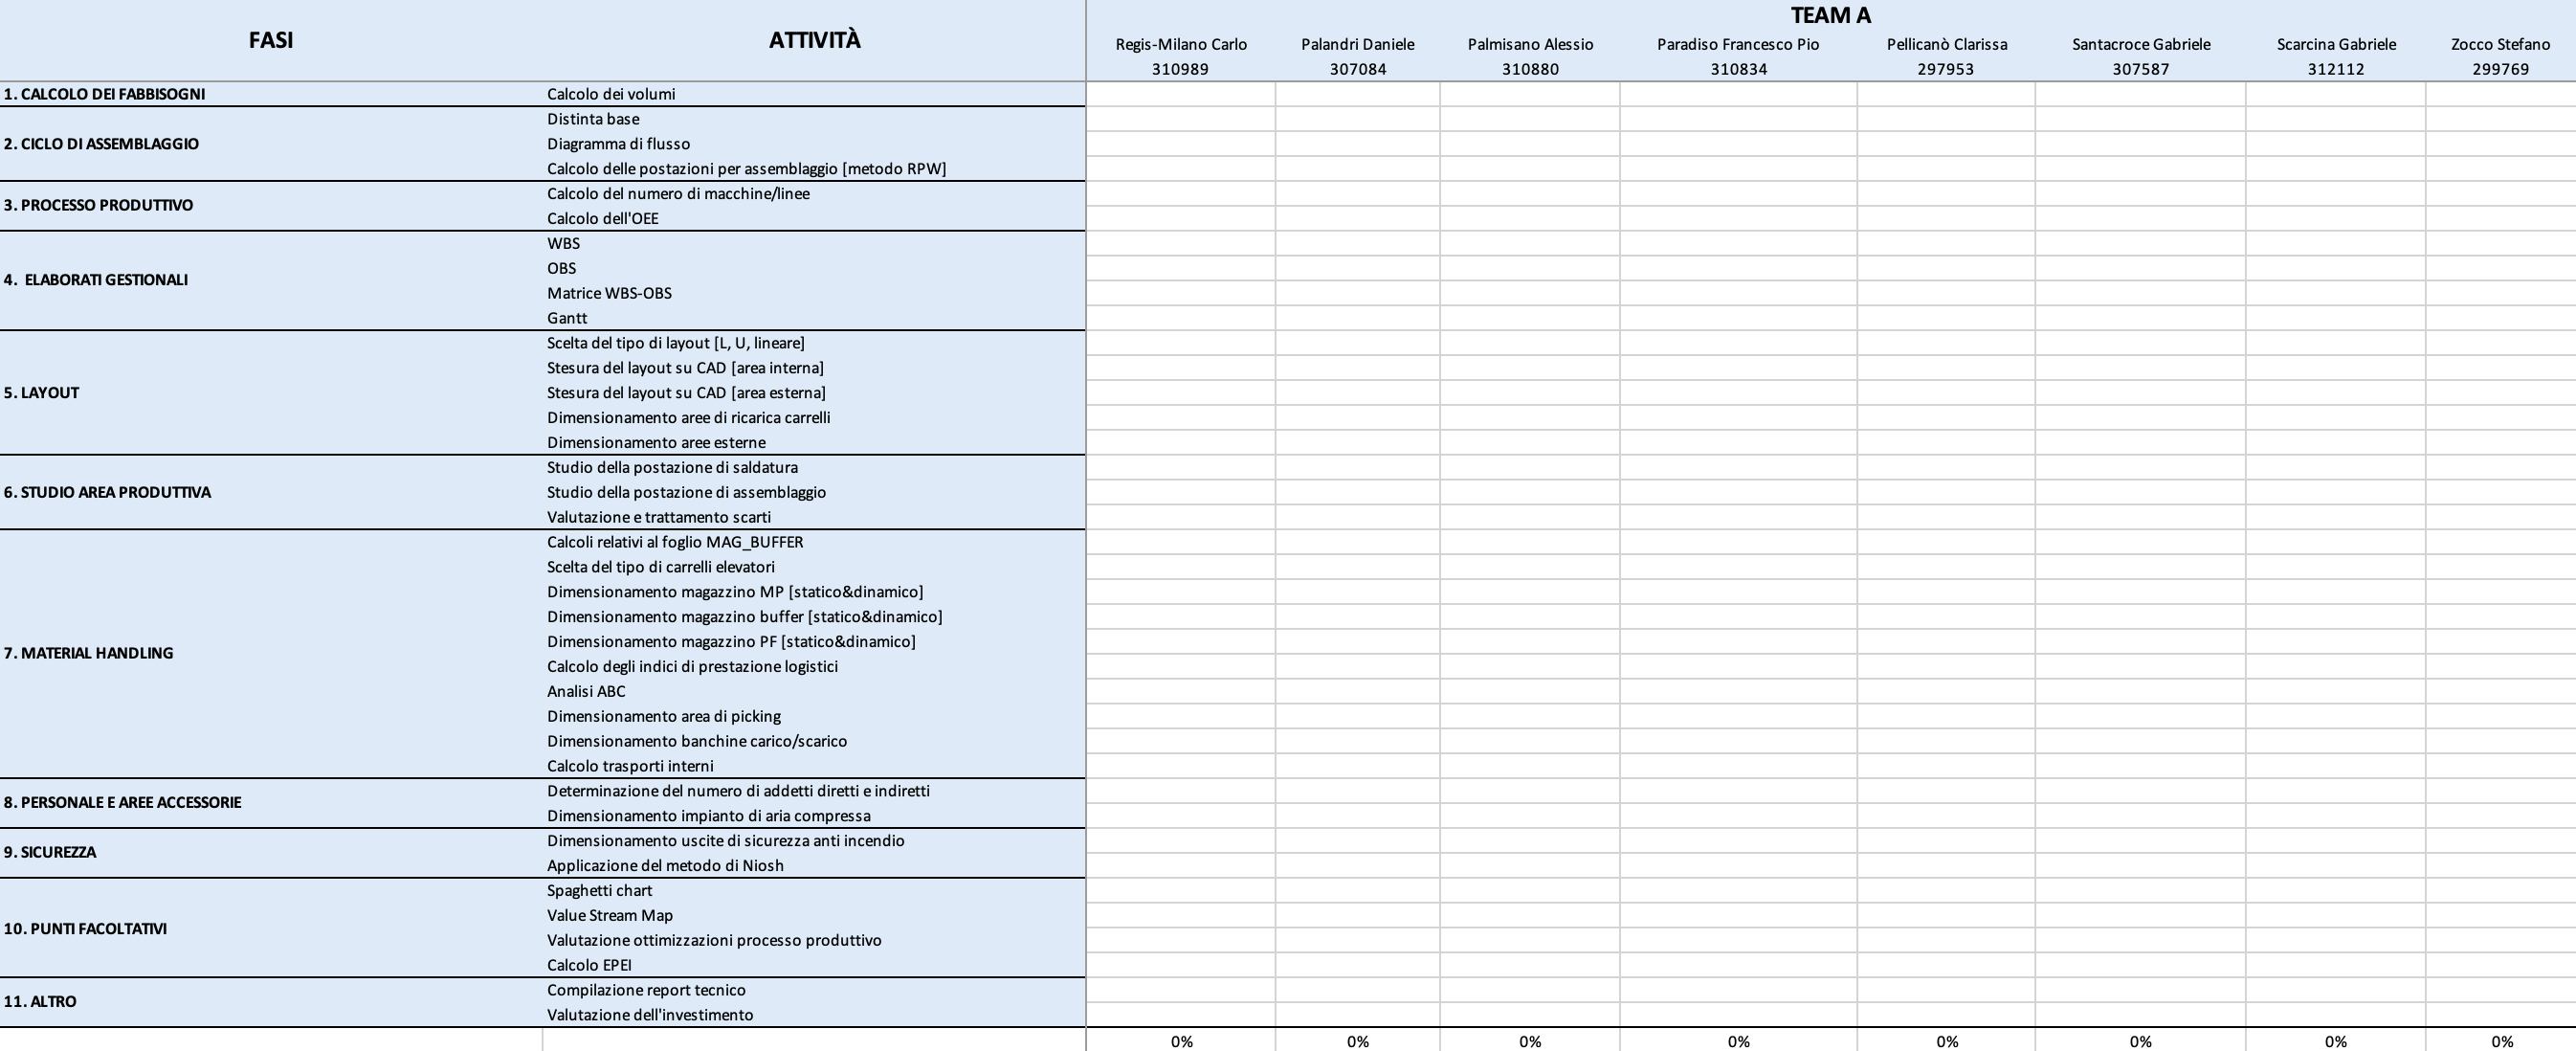
\includegraphics[width=\textwidth]{images/Matrice WBS-OBS.png}
    \caption{Matrice WBS-OBS}
    \label{fig: Matrice WBS-OBS}
\end{figure}

\noindent
È possibile consultare la matrice WBS-OBS completa nell'allegato "{{matriceWBSOBS}}".
\newpage

\subsection{Gantt}
Il diagramma di Gantt è uno strumento di pianificazione che permette di visualizzare le attività del progetto e le loro dipendenze nel tempo.
Di seguito, è riportato un estratto del diagramma di Gantt per il progetto:
\begin{figure} [H]
    \centering
    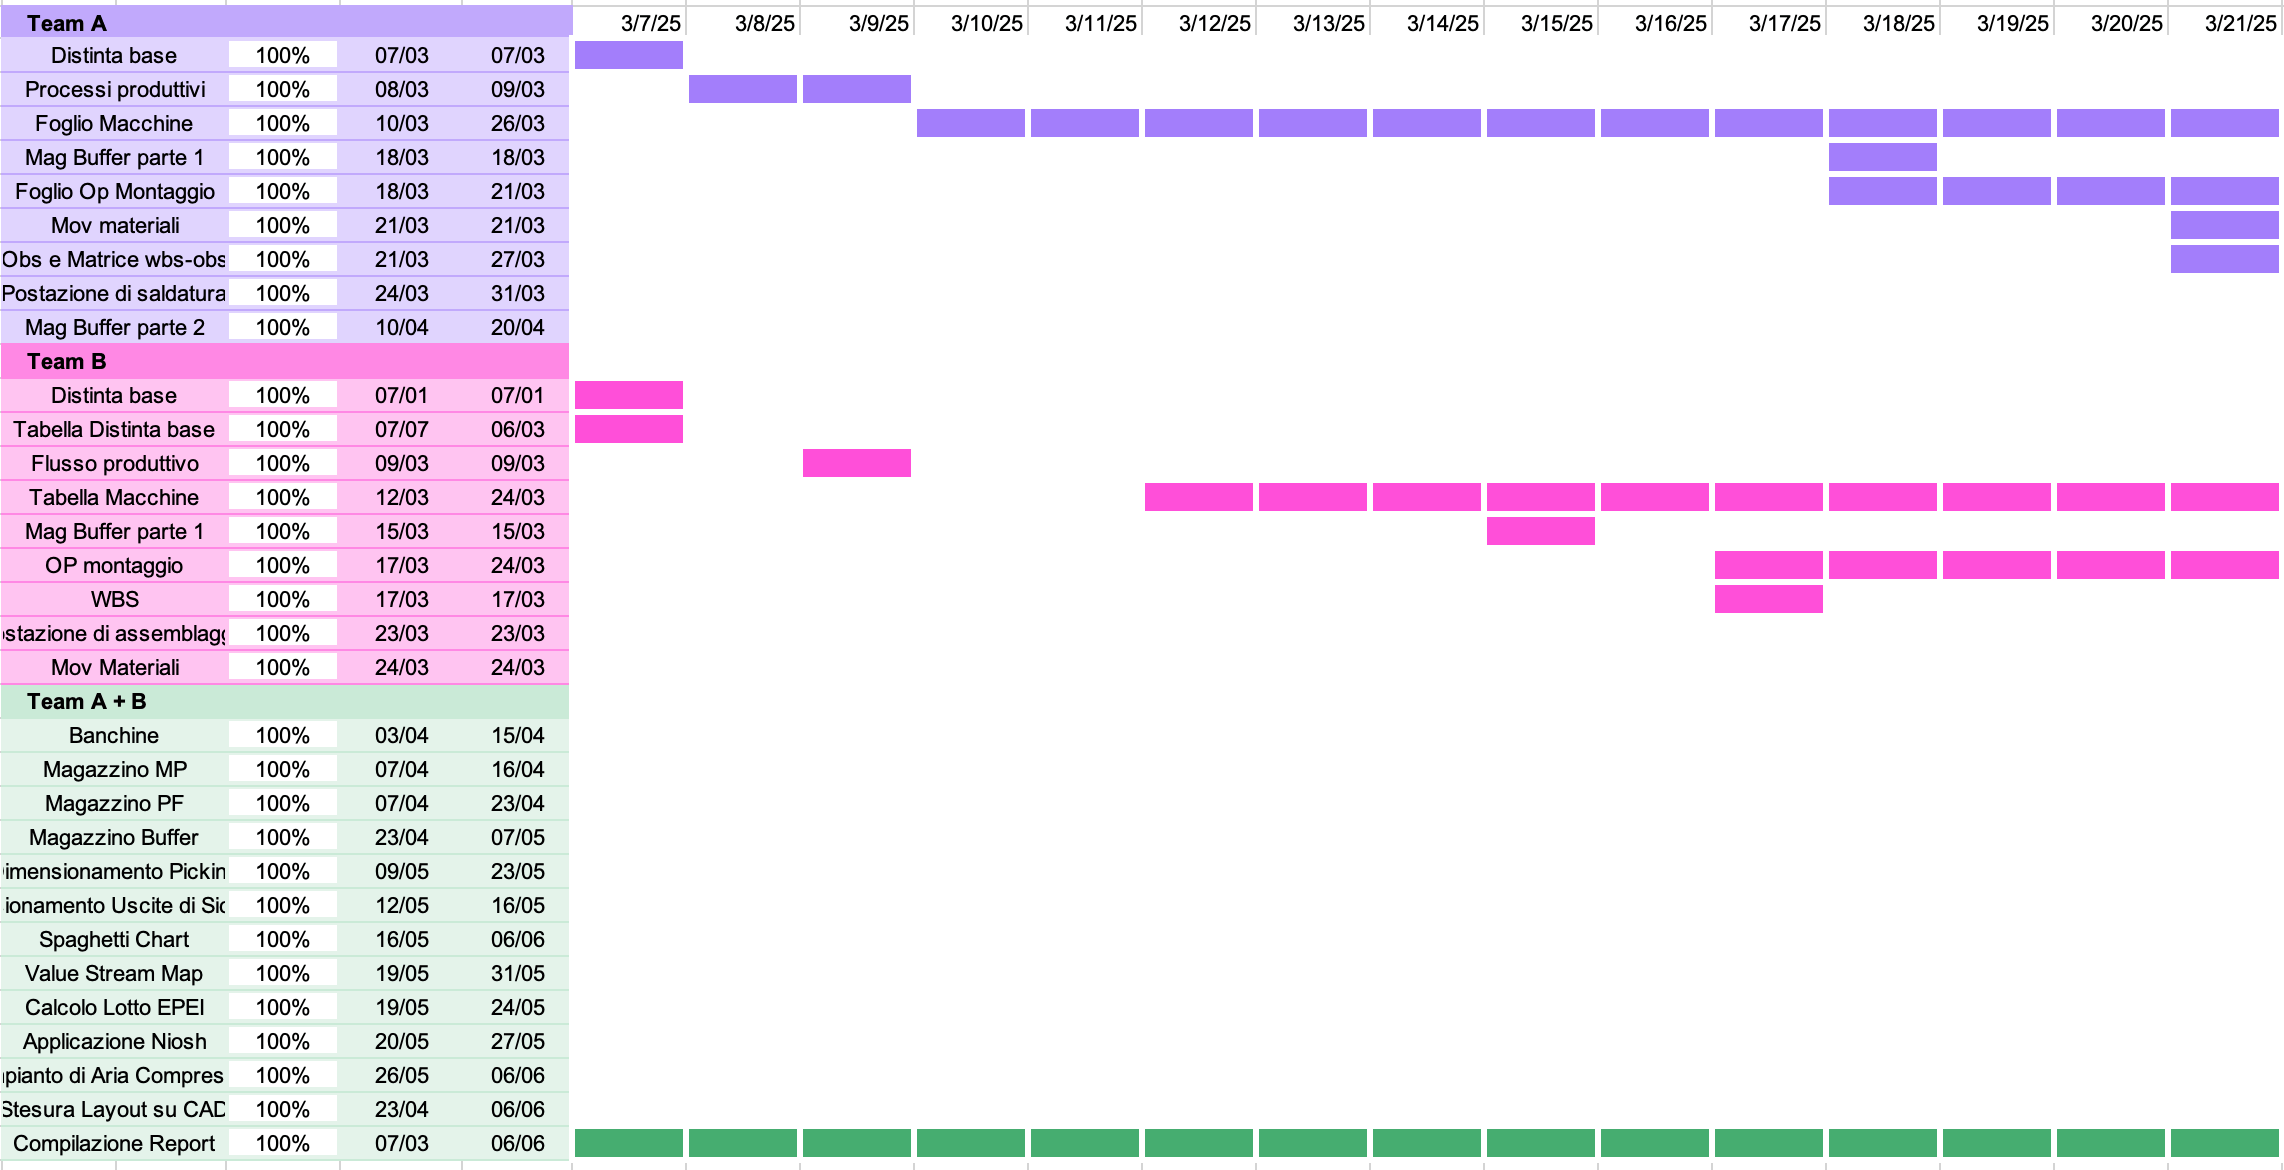
\includegraphics[width=\textwidth]{images/Gantt.png}
    \caption{Diagramma di Gantt}
    \label{fig: Diagramma di Gantt}
\end{figure}

\noindent
Il diagramma di Gantt completo è disponibile nell'allegato "{{gantt}}".
\newpage


\section{Layout}
\subsection{Scelta del tipo di layout [L, U, lineare]}
Il layout scelto preliminarmente era ad "L", successivamente si è deciso di adottare un layout ad "U" per accoppiare in modo più efficiente le aree produttive e logistiche precedentemente dimensionate.

Il layout "lineare" è stato scartato in quanto avrebbe portato a percorrenze molto maggiori, aumentando le distanze tra le linee di assemblaggio ed il magazzino materie prime.
\newpage

\subsection{Stesura del layout su CAD}
\subsubsection{Area interna}
Preliminarmente è stata scelta una maglia di grandi dimensioni (14x28 m), tuttavia questa inficiava negativamente sulla compartimentazione delle diverse aree, creando grossi spazi vuoti.\\
Si è quindi deciso di cambiare schema, adottando un maglia più piccola (12x12 m), quadrata in acciaio, considerando i pilasti con ingombro 40x50 cm.
È possibile consultare il layout dell'area interna nell'allegato "{{areaInterna}}".
\vskip4em

\subsubsection{Area ricarica carrelli}
Per il calcolo delle postazioni di ricarica dei vari mezzi presenti all'interno dello stabilimento è stato considerato lo scenario peggiore possibile, ovvero che tutti i mezzi debbano essere ricaricati contemporaneamente.

Per prima cosa sono state ricavate le varie lunghezze degli automezzi presenti nello stabilimento:
\begin{itemize}
    \item Carrelli elevatori Toyota: $790 \times 2180~\mathrm{mm}$
    \item Carrelli commissionatori: $800 \times 1512~\mathrm{mm}$
    \item Carrelli elevatori Linde: $1600 \times 3208~\mathrm{mm}$
    \item Vagoni carrelli commissionatori: $1070 \times 2069~\mathrm{mm}$
\end{itemize}

In queste tabelle sono presenti anche i vagoni dei commissionatori, poiché inizialmente si era pensato di caricare i carrelli commissionatori con ancora attaccati i vagoni. Tuttavia, questa soluzione è stata successivamente scartata, in quanto occupava troppo spazio.

Successivamente, avendo a disposizione tutte le dimensioni dei vari mezzi e delle batterie ($300 \times 790~\mathrm{mm}$), si sono potuti effettuare i calcoli per ricavare le aree occupate dai mezzi, escludendo i corridoi:
\begin{table} [H]
    \centering
    \renewcommand{\arraystretch}{1.5}
    \begin{tabular}{|l|c|}
        \hline
        \textbf{Mezzo} & \textbf{Area} [$\mathrm{m^2}$] \\
        \hline
    Toyota & 139,1032 \\
    Linde & 0 \\
    Commissionatori & 2,8992 \\
        \hline
        \textbf{Totale} & 142,0024 \\
        \hline
    \end{tabular}
    \caption{Aree occupate senza corridoi}
    \label{tab: Aree occupate senza corridoi}
\end{table}
    
Dopo questo passaggio, i mezzi sono stati disposti sul CAD in una posizione perimetrale dello stabilimento, in modo da consentire l'installazione di eventuali ventole per l'evacuazione dei fumi in caso di incendio. Posizionare questa zona in altre aree sarebbe stato sconveniente.
\vskip1em
È possibile consultare il layout dell'area di ricarica carrelli nell'allegato "{{areaRicarica}}" mentre i calcoli sono disponibili nell'allegato "{{excelCompleto}}".
\newpage

\subsubsection{Area esterna}
\subsubsection*{Parcheggi per automobili}
Per il calcolo dei parcheggi per automobili è stata utilizzata la seguente formula:
\begin{equation}
n_{\text{parcheggi}} = k \cdot n_{\text{dipendenti}}
\end{equation}
\noindent
dove $k$ è un coefficiente compreso tra $0.4$ e $0.6$. Nel nostro caso è stato adottato il valore $k = 0.5$, ottenendo:

\begin{equation}
n_{\text{parcheggi}} = 0.5 \cdot n_{\text{dipendenti}} = 184
\end{equation}
\noindent
Di questi 184 parcheggi, uno ogni 50 deve essere riservato ai disabili. Nel nostro caso, quindi, sono stati previsti:

\begin{equation}
n_{\text{disabili}} = \frac{184}{50} = 4
\end{equation}
\noindent
I parcheggi per disabili hanno una larghezza maggiore, pari a:

\begin{equation}
\text{Larghezza} = 3.2~\mathrm{m}
\end{equation}
\noindent
Le dimensioni dei parcheggi considerate sono:

\begin{itemize}
    \item Parcheggi standard: profondità $= 4.5~\mathrm{m}$, larghezza $= 2.5~\mathrm{m}$
    \item Parcheggi disabili: profondità $= 4.5~\mathrm{m}$, larghezza $= 3.2~\mathrm{m}$
\end{itemize}

\noindent
Nel disegno CAD è stato considerato un numero di parcheggi leggermente superiore, per sovradimensionamento.
\vskip4em

\subsubsection*{Parcheggi per biciclette e motocicli}
La stessa formula è stata utilizzata per il calcolo dei parcheggi per biciclette e motocicli, adottando un coefficiente $k$ compreso tra $0.1$ e $0.15$. Con $k = 0.13$ si è ottenuto:

\begin{equation}
n_{\text{parcheggi bici/moto}} = 0.13 \cdot n_{\text{dipendenti}} = 48
\end{equation}
\noindent
Le dimensioni considerate per ogni parcheggio bici/moto sono:

\begin{itemize}
    \item Profondità $= 2.5~\mathrm{m}$
    \item Larghezza $= 1.4~\mathrm{m}$
\end{itemize}

\noindent
Si ottiene così un'area compresa tra $2$ e $5~\mathrm{m^2}$, in linea con le indicazioni normative.
\newpage

\subsubsection*{Piazzale dei camion}
Per il piazzale dei camion sono stati considerati:

\begin{equation}
\text{Lunghezza piazzale} = 40~\mathrm{m}
\end{equation}
\noindent
frontalmente alle banchine per consentire le manovre. La pendenza del piazzale è stata progettata nel seguente modo:

\begin{itemize}
    \item Nei primi $15~\mathrm{m}$: pendenza $= 2\%$
    \item Nei successivi $25~\mathrm{m}$: pendenza $= 10\%$
\end{itemize}
\noindent
Tale configurazione permette un corretto deflusso delle acque meteoriche verso uno scolo posizionato in prossimità della mezzeria.

Le banchine sono state posizionate ad una distanza di $12~\mathrm{m}$ tra loro.
\vskip2em

\noindent
È possibile consultare il layout dell'area esterna nell'allegato "{{areaParcheggi}}".
\newpage

\subsubsection{Collocazione stabilimento}
L'area scelta per la costruzione del nuovo stabilimento si trova a Fiumicino (RM), precisamente in Via della Corona Boreale 111. Si tratta di una superficie di 10 ettari (100.000 m²), adiacente all'Aeroporto di Fiumicino, a pochi minuti dal porto di Civitavecchia e ben collegata con l'autostrada A91 Roma-Fiumicino; è inoltre inclusa nella Zona Logistica Semplificata (ZLS).

Le ZLS offrono vantaggi come procedure amministrative semplificate e incentivi fiscali per le imprese. Questa zona è strategica per attività logistiche e produttive, grazie alla vicinanza con l'aeroporto internazionale e le principali arterie di trasporto, e per l'insediamento di uno stabilimento industriale nel settore automotive, grazie alla sua posizione privilegiata e alle caratteristiche urbanistiche favorevoli. La posizione garantisce un accesso rapido alle principali infrastrutture di trasporto, facilitando le operazioni logistiche e distributive.

\begin{table}[H]
    \centering
    \renewcommand{\arraystretch}{1.5}
    \resizebox{0.9\textwidth}{!}{
    \begin{tabular}{|l|c|}
        \hline
        \multicolumn{2}{|c|}{\textbf{Coordinate GPS}} \\
        \hline
        Valori & 41.7995° N, 12.2421° E \\
        \hline
        \multicolumn{2}{|c|}{\textbf{Collegamenti e distanze}} \\
        \hline
        Aeroporto di Fiumicino & ~2 km \\
        Porto di Civitavecchia & ~60 km \\
        Stazione ferroviaria di Fiumicino Aeroporto & ~3 km \\
        Autostrada A91 (Roma-Fiumicino) & ~2 km \\
        Grande Raccordo Anulare (GRA) & ~10 km \\
        \hline
        \multicolumn{2}{|c|}{\textbf{Conformità urbanistica e ambientale}} \\
        \hline
        Zona Sismica & 3B (pericolosità sismica bassa) \\
        Indice di edificabilità & 25\% (fino a 25.000 m² coperti, altezza max 15 m) \\
        Prezzo & €6.000.000 \\
        \hline
    \end{tabular}
    }
    \caption{Dettagli del terreno}
    \label{tab:dettagli_terreno}
\end{table}

\begin{figure}[H]
    \centering
    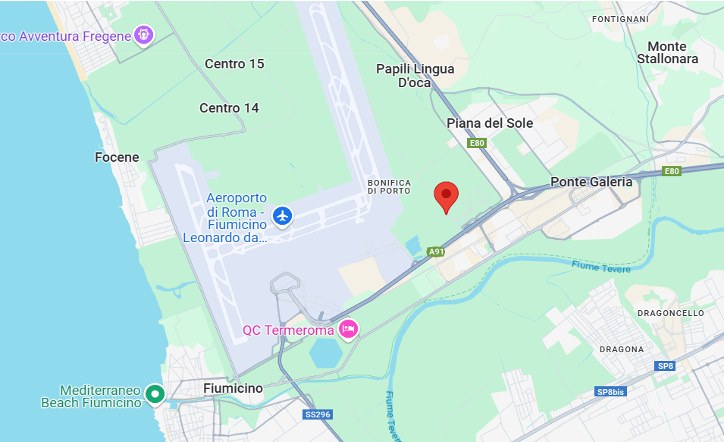
\includegraphics[width=0.8\textwidth]{images/Collocazione stabilimento.png}
    \caption{Collocazione stabilimento}
    \label{fig: Collocazione stabilimento}
\end{figure}

È possibile consultare l'ortografia di ubicazione dell'impianto nell'allegato "{{collocazioneStabilimento}}".
\newpage

\subsection{Dimensionamento aree produttive}
\subsubsection{Indici di prestazione logistici}
Gli indici di prestazione logistici sono stati così calcolati:
\begin{align*}
    & I_\text{eff} = \frac{A_\text{eff}}{\text{UDC}_{rich}} \\
    & I_\text{eff,vol} = I_\text{eff} \times N_\text{liv,max} \times h_\text{vano} \\
    & \text{PR}_\text{eff} = \sum N_\text{vani} \\
    & S_\text{DT} = \frac{N_\text{liv,DT}}{N_\text{liv,DT} \times D_\text{righe}}
\end{align*}

\noindent
dove:
\begin{itemize}
    \item $I_\text{eff}$ = impronta effettiva
    \item $A_\text{eff}$ = area effettiva
    \item $\text{UDC}_{rich}$ = unità di carico richieste
    \item $I_\text{eff,vol}$ = impronta effettiva volumetrica
    \item $N_\text{liv,max}$ = numero massimo di livelli
    \item $h_\text{vano}$ = altezza del vano
    \item $\text{PR}_\text{eff}$ = potenzialità ricettiva effettiva
    \item $N_\text{vani}$ = numero di vani
    \item $S_\text{DT}$ = selettività drive-through
    \item $N_\text{liv,DT}$ = numero di livelli drive-through
    \item $D_\text{righe}$ = dimensione delle righe
\end{itemize}

\vskip2em
\noindent
I risultati ottenuti sono i seguenti:
\begin{table} [H]
    \centering
    \renewcommand{\arraystretch}{1.5}
    \begin{tabular}{|l|c|c|}
        \hline
        \textbf{Indice} & \textbf{Valore} & \textbf{Unità} \\
        \hline
        $I_\text{eff}$ & 0.708 & $m^2/UdC$ \\
        $I_\text{eff,vol}$ & 4.049 & $m^3/UdC$ \\
        $\text{PR}_\text{eff}$ & 4992 & UdC \\
        $S_\text{DT}$ & 11.11 & $\%$ \\
        \hline
    \end{tabular}
    \caption{Indici di prestazione logistici}
    \label{tab: Indici di prestazione logistici}
\end{table}
\newpage


\section{Studio area produttiva}
\subsection{Studio della postazione di saldatura}
L'area di saldatura è stata dimensionata tenendo conto della necessità di percorsi pedonali di accesso ai box di minimo 80 cm, i box sono stati posizionati in linee da 5 ciascuna, per un totale di 10 Box.

Di fronte a ciascun box, alla distanza minima possibile per evitare lunghi tragitti per l'operatore, si trovano le unità di carico in entrata (corpo e inserto plancia) e in uscita (corpo+inserto plancia e scarti).

È possibile consultare il layout della postazione di saldatura nell'allegato "{{layoutPostazioneSaldatura}}".
\vskip4em

\subsection{Studio della postazione di assemblaggio}
Per le linee di assemblaggio, queste sono state disposte in linea e poi raccordate per categoria di prodotto in un'unica linea di rulli motorizzati, che portano i pezzi finiti ad un pallettizzatore posto in fondo alla linea.

Le linee di rulli motorizzati che si dovessero trovare affiancate sono distanziate di 60 cm per consentire eventuali interventi manutentivi.

Ogni postazione è composta da un tavolo di lavoro e un'area in cui si troverà l'operatore, di 2 $m^2$, ogni tavolo è distanziato dal rullo di 20 cm per evitare trasmissione di vibrazioni da parte dello stesso.

Le postazioni sono distanziate tra loro in modo da consentire che l'operatore possa prelevare il pezzo dalla linea agevolmente.

A monte della linea è posto un braccio robotico al fine di caricare sui rulli la plancia, i kit e il cupolotto.

È possibile consultare il layout della postazione di assemblaggio nell'allegato "{{layoutPostazioneAssemblaggio}}".
\vskip4em

\subsection{Valutazione e trattamento scarti}
Per gestire gli scarti si è deciso di triturarli in apposito trituratore di cui si allegano le specifiche tecniche.\\
Per lo stoccaggio degli stessi si è deciso di utilizzare sacchi industriali di tipo \textit{big bag} e di sfruttare le corsie che si disimpegnano nel magazzino materie prime man mano che la produzione procede per riporli.\\
Infine, per lo smaltimento si pensava di riconsegnare i sacchi industriali ai camion provenienti dal fornitore dei prodotti stampati, per il riciclo degli stessi.
\newpage

\section{Material handling}
\subsection{Calcoli relativi al foglio MAG BUFFER}
\subsubsection{Indice di rotazione}
Per definire i vari magazzini quali quello delle materie prime, prodotti finiti e semilavorati, sono state definite diverse grandezze che hanno permesso la costruzione di una tabella che evidenzia, in una prima parte, i fabbisogni mensili e, in una seconda parte, la capacità dei magazzini e buffer.
\begin{figure} [H]
    \centering
    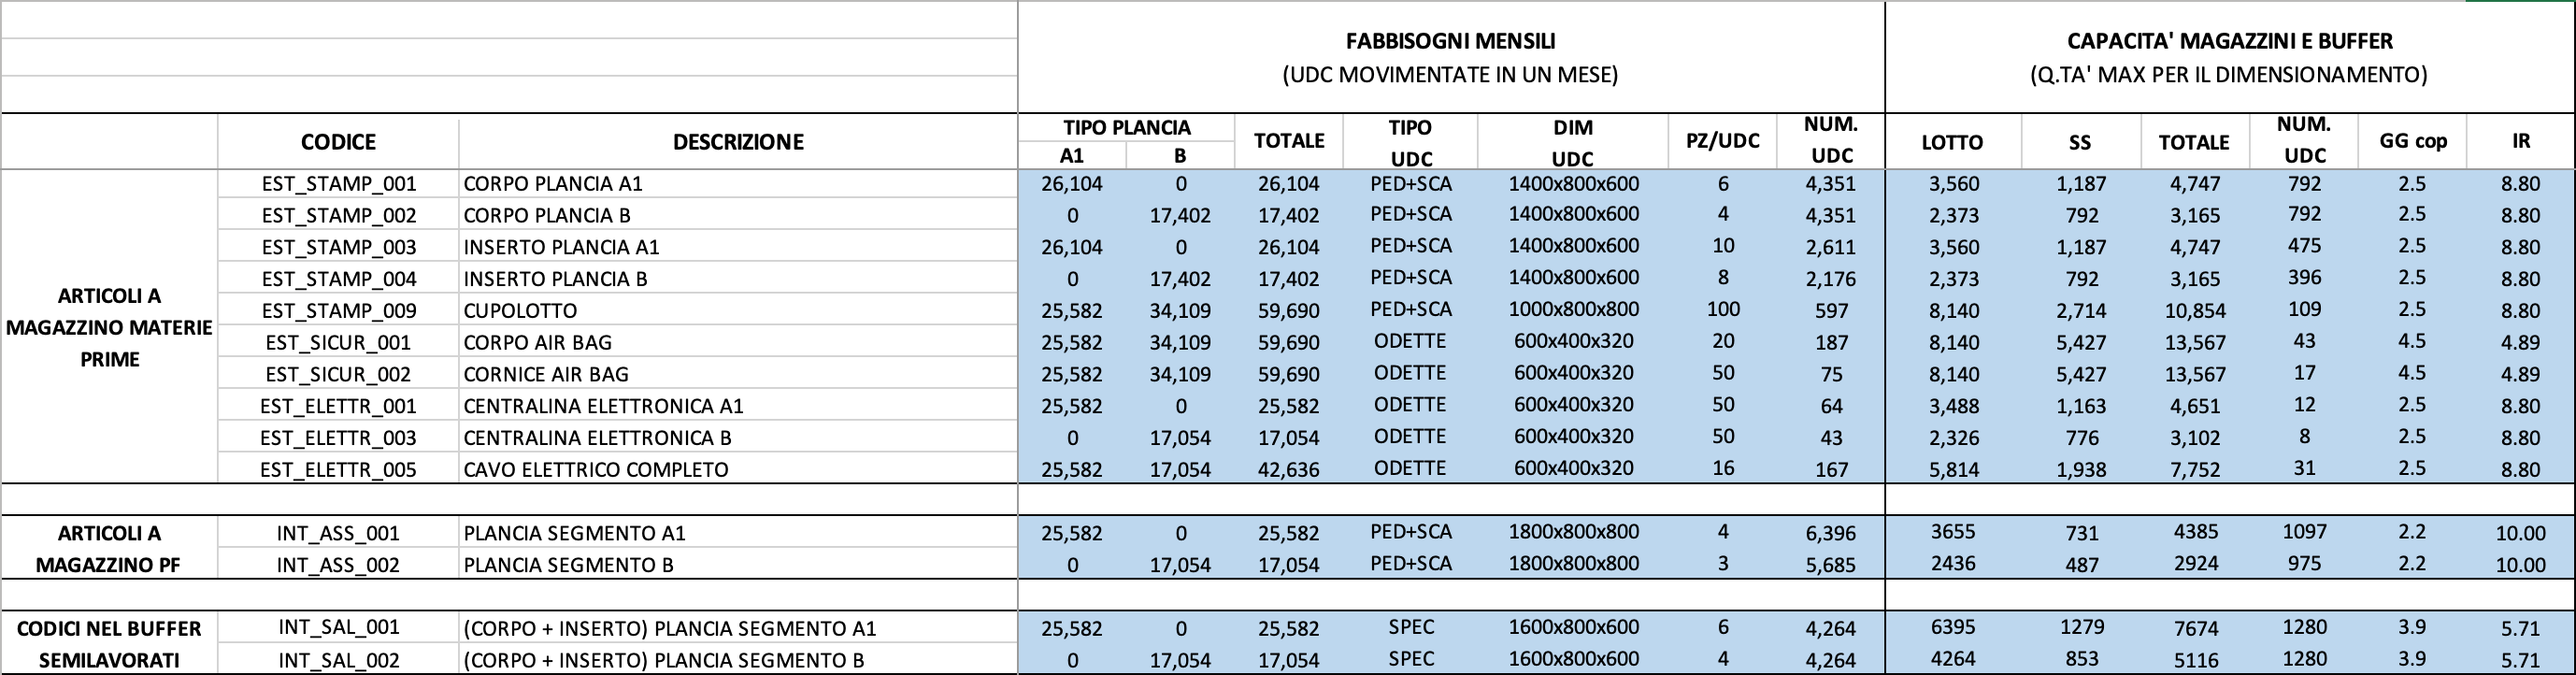
\includegraphics[width=\textwidth]{images/Magazzini.png}
    \caption{Magazzini}
    \label{fig: Magazzini}
\end{figure}

\subsubsection{Fabbisogni mensili}
Come prima cosa, è stato calcolato il numero di pezzi a seconda della tipologia di plancia per poi farne la somma per ciascun componente:
\begin{equation}
    N_\text{pezzi,lordi,tot} = N_\text{pezzi,lordi,A1} + N_\text{pezzi,lordi,B}
\end{equation}

Successivamente, dopo la definizione della tipologia di UdC, delle sue dimensioni e del numero di pezzi per UdC dalle prescrizioni iniziali, viene calcolato il numero di UdC in due modalità differenti a seconda della tipologia di UdC:
\begin{align}
    & \text{UdC} 
    && N_\text{udc} = \frac{N_\text{pezzi,lordi,tot}}{N_\text{pezzi/udc}} 
    \\
    & \text{ODETTE} 
    && N_\text{odette} = \frac{N_\text{pezzi,lordi,tot}}{N_\text{pezzi/udc}\cdot N_\text{odette/piano}\cdot I }
\end{align}
dove:
\begin{itemize}
    \item $N_\text{odette/piano}$ = numero di ODETTE per ogni piano di un pallet
    \item $I$ = impilabilità (prescrizioni iniziali)
\end{itemize}

\newpage

\subsubsection{Capacità dei magazzini e buffer}
Per questa parte della tabella del magazzino delle materie prime, è stata calcolata la somma fra il numero di lotti e la scorta di sicurezza, entrambi calcolati come segue:
\begin{equation}
    N_\text{lotti} = \frac{N_\text{pezzi,lordi,tot}}{N_\text{giorni,MM}\cdot \text{Int}_R}
\end{equation}

\begin{equation}
    \text{SS} = \text{ceiling}\left(\frac{N_\text{pezzi,lordi,tot}}{N_\text{giorni,MM}} \cdot \text{coeff}_\text{SS}\right)
\end{equation}

dove:
\begin{itemize}
    \item $N_\text{giorni,MM}$ = numero di giorni lavorativi mensili
    \item $\text{Int}_R$ = intervallo di riordino (prescrizioni iniziali)
    \item $\text{coeff}_\text{SS}$ = \text{coefficiente scorta di sicurezza (prescrizioni iniziali)}
\end{itemize}

Successivamente, è stato calcolato il numero di UdC in due modalità distinte in funzione della tipologia di UdC:
\begin{align}
    & \text{UdC} 
    && N_\text{udc} = \frac{N_\text{lotti}+\text{SS}}{N_\text{pezzi/udc}} 
    \\
    & \text{ODETTE} 
    && N_\text{odette} = \frac{N_\text{lotti}+\text{SS}}{N_\text{pezzi/udc}\cdot N_\text{odette/piano}\cdot I }
\end{align}

Dopo questi calcoli, sono stati definiti i giorni di copertura come:
\begin{equation}
    \text{GG}_\text{cop} = \frac{\text{IR}+2\cdot \text{coeff}_\text{SS}}{2}
\end{equation}

Infine, è stato possibile calcolare l'indice di rotazione come:
\begin{equation}
    \text{IR} = \frac{N_\text{giorni,MM}}{\text{GG}_\text{cop}}
\end{equation}
\newpage

\subsection{Scelta del tipo di carrelli elevatori}
Per confrontare le configurazioni bifrontale e drive-through nei magazzini sono stati scelti due tipi di carrelli, rispettivamente uno a forche trilaterali e uno per corsie strette.
\vskip2em

Ai fini della standardizzazione del modello di carrello elevatore e poiché la scelta dei magazzini è ricaduta sulla scaffalatura drive-thrugh è stato scelto il carrello per corsie strette BT-STAXIO SERIE S TOYOTA (documentazione dell'elevatore disponibile nell'allegato "{{elevatoreBTSTAXIO}}").
Questo carrello è l'unico in grado di accedere alle corsie del magazzino materie prime, in quanto è largo solo 80 cm.
\vskip2em

Per le aree di carico e scarico dei camion sono stati scelti i transpallet manuali BT-LIFTER SERIE L TOYOTA (documentazione del transpallet disponibile nell'allegato "{{transpalletBTLIFTER}}").
\newpage

\subsection{Dimensionamento magazzino MP}
Per il dimensionamento statico dei magazzini materie prime, buffer e prodotti finiti, si è scelto di fare un trade off su dimensioni e investimento complessivo considerando il costo della superficie, dai vani e dei carrelli.
Si è scelto di fare i calcoli in riferimento ad una configurazione bifrontale, con carrello a forche trilaterali, e un drive through, con carrello per corsie strette.

\subsubsection{Magazzino Bifrontale}
Per il dimensionamento del modulo base degli stampati, si è scelto un vano di dimensione 1550x950x950 mm, mentre per i pallet di odette, un vano di dimensioni 1350x950x1430 mm.

\paragraph{Dimensionamento statico}\mbox{}\\
Per il dimensionamento statico si procede come segue:
\begin{align}
    & A_\text{MB} = a\,(2b+c) \\
    & N_\text{livelli} = \text{int}\left(\frac{\text{12˙000}}{H_\text{soll,for}}\right)+1 \\
    & N_\text{UdC/MB} = 2 \cdot N_\text{livelli} \\
    & I_{th} = \frac{A_\text{MB}}{N_\text{UdC/MB}} \\
    & A_\text{compl,th} = I_{th} \cdot \text{PR} \\
    & U_\text{id} = \sqrt{2 \cdot A_\text{compl,th}} \\
    & V_\text{id} = 2\cdot U_\text{id} \\
    & N_\text{corr} = \frac{U_\text{id}}{L_\text{MB}} \\
    & N_\text{MB/corr} = \text{ceiling}\left(\frac{\text{PR}}{N_\text{corr} \cdot N_\text{UdC/MB}}\right) \\
    & \text{PR}_\text{eff} = N_\text{UdC/MB} \cdot N_\text{corr} \\
    & U_\text{eff} = (N_\text{corr} \cdot L_\text{MB}) + 6 \\
    & V_\text{eff} = (N_\text{MB/corr} \cdot a) + 6 \\
    & A_\text{eff} = U_\text{eff} \cdot V_\text{eff}
\end{align}
\noindent
dove:
\begin{itemize}
    \item $A_\text{MB}$ = area del modulo base
    \item $a$ = lunghezza del vano
    \item $b$ = larghezza del vano
    \item $c$ = altezza del vano

    \item $N_\text{livelli}$ = numero di livelli
    \item $H_\text{soll,for}$ = altezza sollevamento forche

    \item $N_\text{UdC/MB}$ = numero di UdC per modulo base
    
    \item $I_{th}$ = impronta teorica

    \item $A_\text{compl,th}$ = area complessiva teorica
    \item $\text{PR}$ = portata reale
    
    \item $U_\text{id}$ = unità ideale

    \item $V_\text{id}$ = volume ideale

    \item $N_\text{corr}$ = numero di corridoi
    \item $L_\text{MB}$ = lunghezza del modulo base
    
    \item $N_\text{MB/corr}$ = numero di moduli base per corridoio
    
    \item $\text{PR}_\text{eff}$ = portata reale effettiva

    \item $U_\text{eff}$ = unità effettive
    \item $V_\text{eff}$ = volume effettivo
    \item $A_\text{eff}$ = area effettiva
\end{itemize}

\begin{figure} [H]
    \centering
    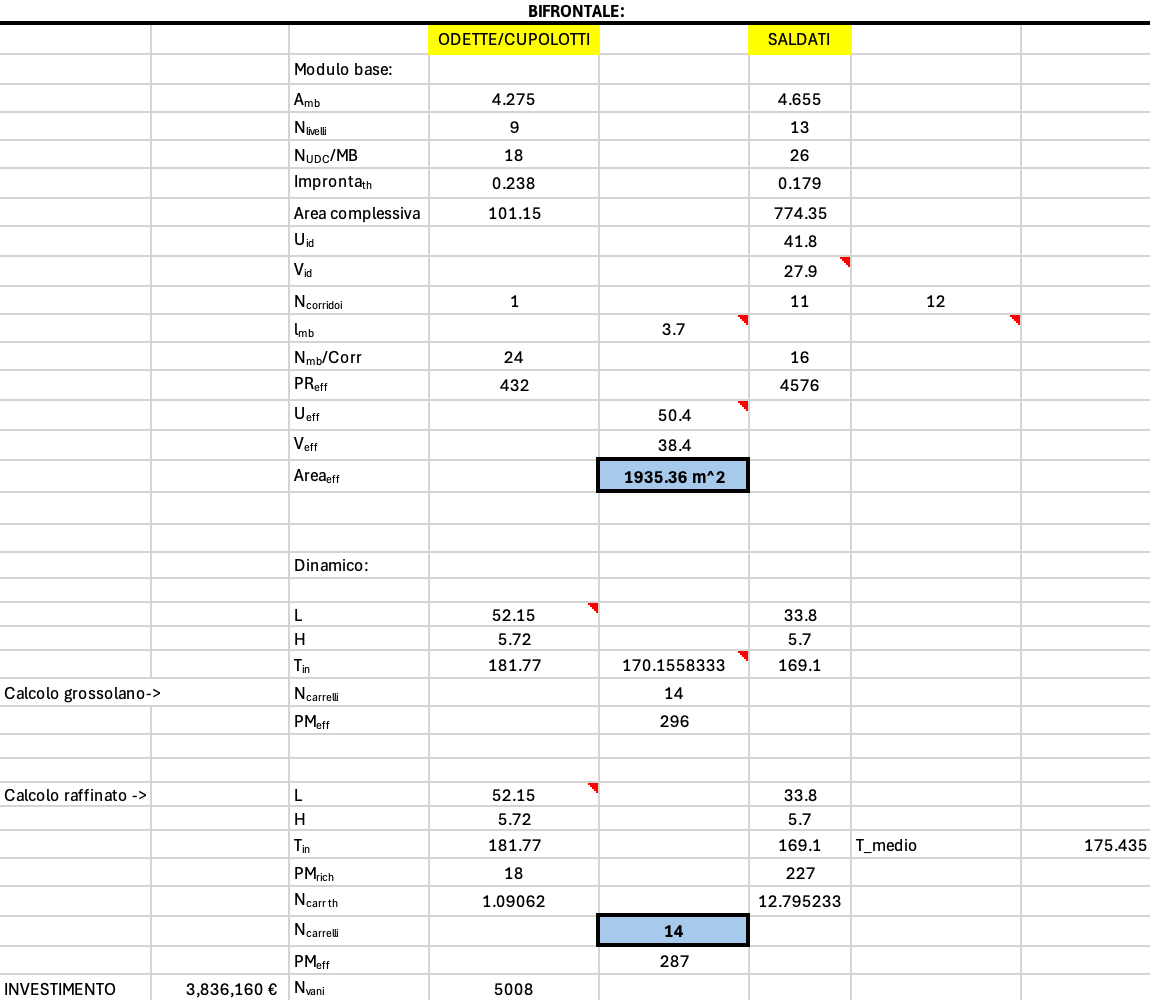
\includegraphics[width=\textwidth]{images/Dimensionamento statico magazzino bifrontale MP.png}
    \caption{Dimensionamento statico magazzino bifrontale materie prime}
    \label{fig: Dimensionamento statico magazzino bifrontale MP}
\end{figure}
\newpage

\subsubsection{Magazzino Drive-Through}
\paragraph{Dimensionamento statico}\mbox{}\\
Per i calcoli relativi al magazzino drive through, a cui si dedicano tutti i prodotti saldati, si cerca di ottenere la massima saturazione possibile per ogni corsia, poichè ognuna di esse è dedicata ad un codice specifico, variando il numero di udc per riga. Scelto tale numero e calcolato il numero di livelli $N_\text{livelli}$, si possono calcolare il numero di righe da assegnare a ciascun codice:
\begin{equation}
    N_\text{rig} = \text{ceiling}\left(\frac{N_\text{UdC}}{N_\text{liv} \cdot N_\text{UdC/rig}}\right)
    \qquad
    \begin{cases}
        N_\text{UdC} = \text{numero di UdC} \\
        N_\text{liv} = \text{numero di livelli} \\
        N_\text{UdC/rig} = \text{numero di UdC per riga}
    \end{cases}
\end{equation}

I codici ODETTE, viste la notevole differenza di dimensioni rispetto ai vani dei saldati, sono stati allocati in una corsia di sole scaffalature bifrontali.
Dopo questi calcoli si procede a disporre le righe ottenute e la scaffalatura bifrontale, tenendo anche conto della presenza di corridoi principali e secondari, sufficienti affinchè il carrello elevatore possa fare una svolta di 90° per entrare ed uscire dalle corsie.
\newpage

\paragraph{Dimensionamento dinamico}\mbox{}\\
Per il dimensionamento dinamico, si calcolano i percorsi di traslazione medi per ODETTE e saldati separatamente, poi si procede come segue:
\begin{align}
    & H = h_v \cdot \frac{N_\text{liv}-1}{2} \\
    & T_\text{in} = 2\left(\frac{L}{V_\text{trasl}}\right)+\frac{H}{V_\text{soll}}+\frac{H}{V_\text{disc}}+2\cdot t_f \\
    & N_\text{carr} = \text{ceiling}\left(\frac{\text{PM} \cdot k \cdot T_\text{in}}{3600}\right)
\end{align}

\noindent
dove:
\begin{itemize}
    \item $H$ = altezza di sollevamento
    \item $h_v$ = altezza del vano
    \item $N_\text{liv}$ = numero di livelli
    \item $T_\text{in}$ = tempo di ingresso
    \item $L$ = percorso medio di un carrello elevatore
    \item $H$ = altezza di sollevamento
    \item $V_\text{trasl}$ = velocità di traslazione
    \item $V_\text{soll}$ = velocità di sollevamento forche
    \item $V_\text{disc}$ = velocità di discesa forche
    \item $t_f$ = tempi fissi
    \item $N_\text{carr}$ = numero di carrelli
    \item PM = potenzialità di movimentazione richiesta
    \item k = coefficiente di saturazione
\end{itemize}

\begin{figure} [H]
    \centering
    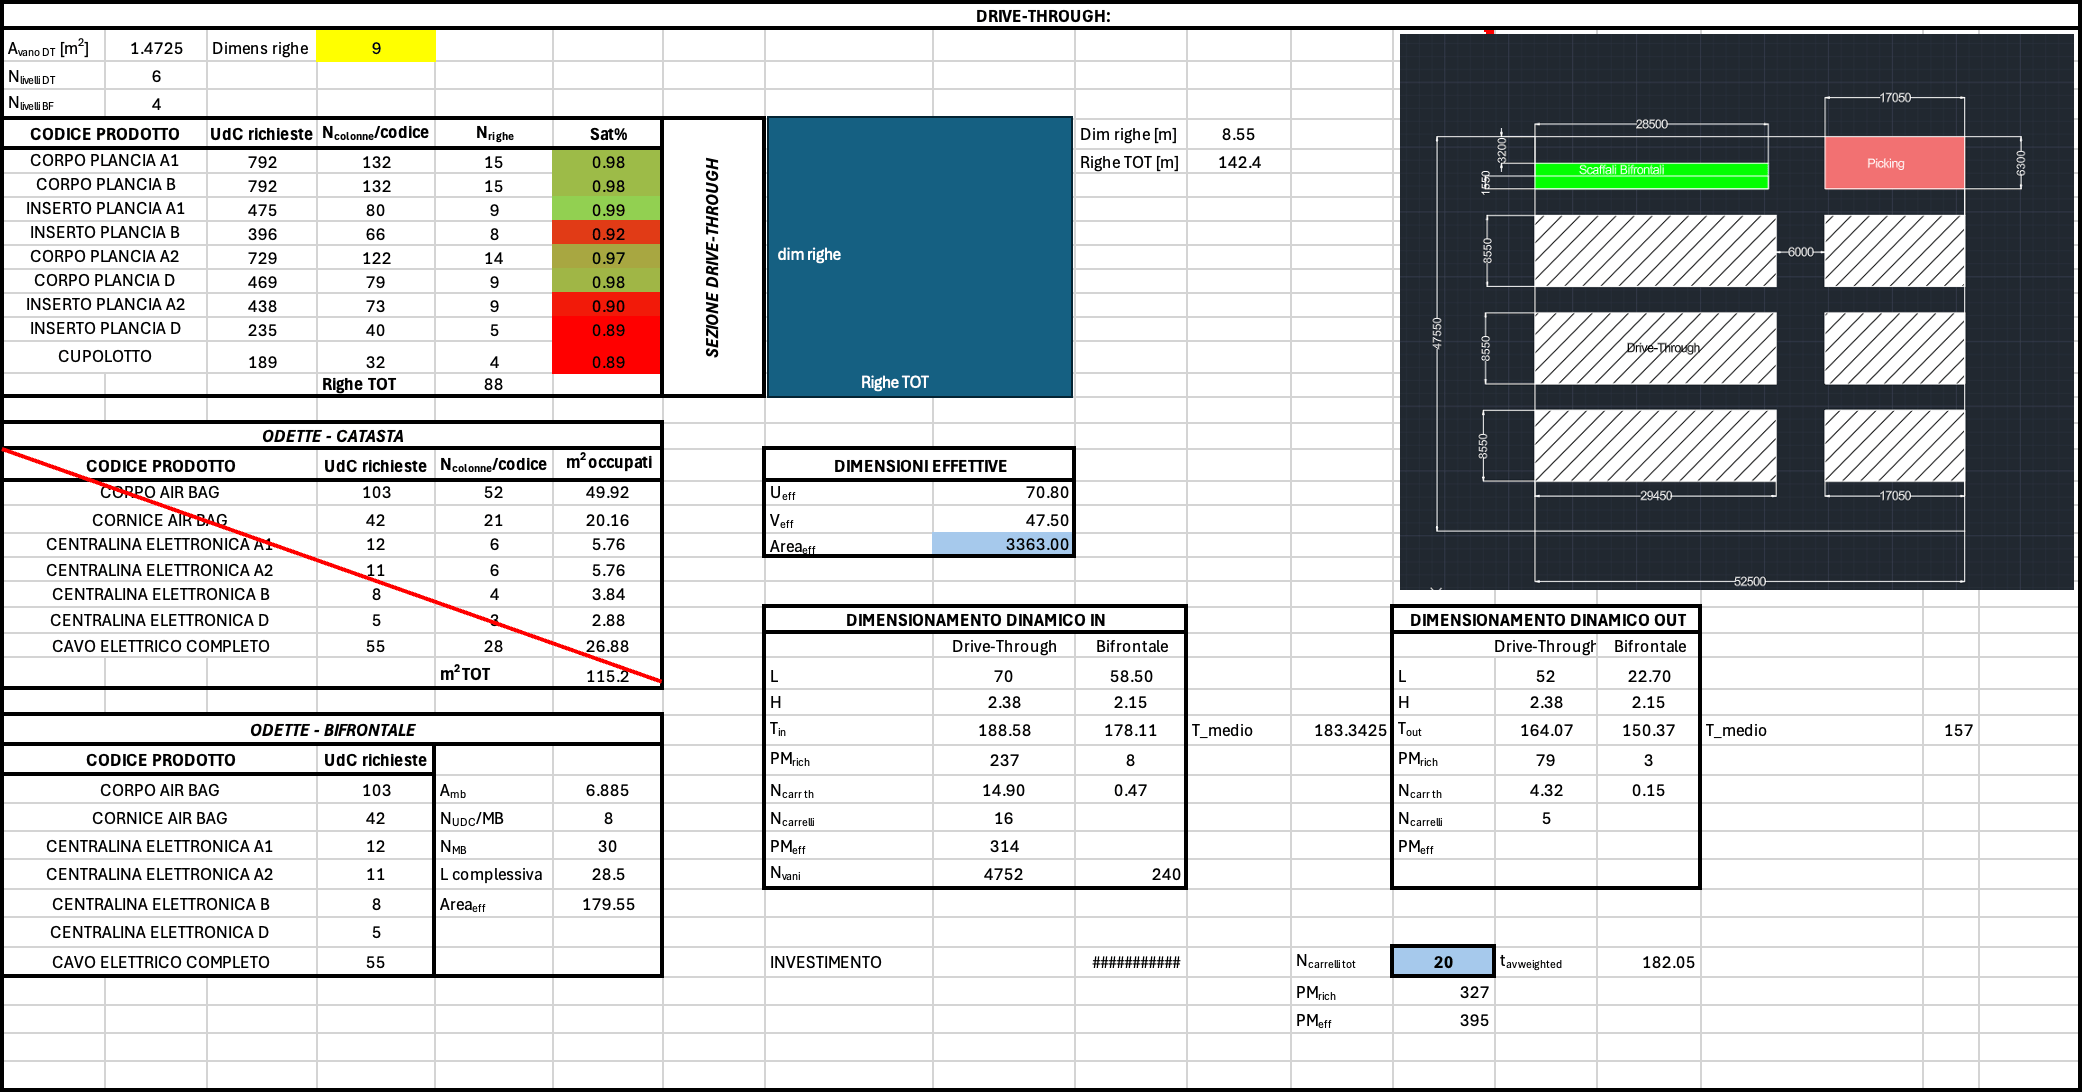
\includegraphics[width=\textwidth]{images/Dimensionamento dinamico magazzino drive-through MP.png}
    \caption{Dimensionamento dinamico magazzino drive-through materie prime}
    \label{fig: Dimensionamento dinamico magazzino drive-through MP}
\end{figure}

\noindent
Tutti i calcoli possono essere consultati nell'allegato "{{excelCompleto}}".
\newpage

\subsection{Dimensionamento magazzino BUFFER}
\subsubsection{Magazzino Bifrontale}
Date le dimensioni del vano 1750x950x750 mm (ottenute sommando 150 mm ai valori dimensionali dell'UDC) si sono potuti effettuare i calcoli sulle dimensioni del modulo base.
Prendendo come riferimento un'altezza massima di 12 m di sollevamento forche del carrello elevatore si è proceduto con il calcolo del numero di livelli e, data la conformazione della scaffalatura bifrontale si è potuto calcolare il numero di unità di carico presenti in ogni modulo base. Tramite l'impronta teorica e la potenzialità ricettiva si è calcolata l'area del magazzino teorica e, in seguito, le dimensioni dei due lati considerando un k pari a 4, un punto di input/output posizionato alla mezzeria del lato maggiore e un'allocazione casuale delle UDC.
\begin{align}
    & L_\text{MB} = 2 \cdot L_\text{vano} + L_\text{corridoio} \\
    & A_\text{MB} = L_\text{MB} \cdot P_\text{vano} \\
    & N_\text{livelli} = \text{int}\left(\frac{12000}{H_\text{vano}}\right) + 1 \\
    & N_\text{UDC} = 2 \cdot N_\text{livelli} \\
    & A_\text{UDC} = \frac{A_\text{MB}}{N_\text{UDC}} \\
    & A_\text{mag} = \text{PR} \cdot A_\text{UDC} \\
    & U_\text{id} = \sqrt{\frac{k}{2} \cdot A_\text{mag}} \\
    & V_\text{id} = \frac{U_\text{id}}{2}
\end{align}
dove:
\begin{itemize}
    \item $L_\text{MB}$ = lunghezza del modulo base
    \item $L_\text{vano}$ = lunghezza base del vano
    \item $L_\text{corridoio}$ = larghezza del corridoio
    \item $A_\text{MB}$ = area del modulo base
    \item $P_\text{vano}$ = profondità del vano
    \item $N_\text{livelli}$ = numero di livelli
    \item $H_\text{vano}$ = altezza del vano
    \item $N_\text{UDC}$ = numero di unità di carico
    \item $A_\text{UDC}$ = area dell'unità di carico
    \item $A_\text{mag}$ = area del magazzino
    \item $\text{PR}$ = potenzialità ricettiva
    \item $U_\text{id}$ = lato orizzontale magazzino ideale
    \item $V_\text{id}$ = lato verticale magazzino ideale
\end{itemize}

\noindent
Il dimensionamento statico e dinamico sono stati effettuati considerando una configurazione del magazzino Haircomb.
\newpage

\paragraph{Dimensionamento statico}\mbox{}\\
Per quanto concerne il dimensionamento statico i calcoli effettuati sono predisposti all'ottenimento dell'area effettiva del magazzino e della dimensione dei due lati. Il dimensionamento è verificato quando la potenzialità ricettiva effettiva è maggiore di quella considerata inizialmente.
\begin{align}
    & N_\text{corr,sec} = \text{ceil}\left(\frac{U_\text{id}}{L_\text{MB}}\right) \\
    & N_\text{mb/corr} = \text{ceil}\left(\frac{\text{PR}}{N_\text{corr,sec} \cdot N_\text{UDC}}\right) \\
    & \text{PR}_\text{eff} = N_\text{UDC} \cdot N_\text{corr,sec} \cdot N_\text{MB/corr} \\
    & U_\text{eff} = N_\text{corr,sec} \cdot L_\text{MB} + L_\text{corr,princ} \\
    & V_\text{eff} = P_\text{vano} \cdot N_\text{MB/corr} + L_\text{corr,princ} \\
    & A_\text{Mag,eff} = U_\text{eff} \cdot V_\text{eff}
\end{align}
dove:
\begin{itemize}
    \item $N_\text{corr,sec}$ = numero di corridoi secondari
    \item $U_\text{id}$ = lato orizzontale magazzino ideale
    \item $L_\text{MB}$ = larghezza del modulo base
    \item $N_\text{mb/corr}$ = numero di moduli base per corridoio
    \item $\text{PR}$ = potenzialità ricettiva
    \item $N_\text{UDC}$ = numero di unità di carico
    \item $\text{PR}_\text{eff}$ = potenzialità ricettiva effettiva
    \item $N_\text{MB/corr}$ = numero di moduli base per corridoio
    \item $U_\text{eff}$ = lato orizzontale magazzino effettivo
    \item $L_\text{corr,princ}$ = lunghezza del corridoio principale (6 metri)
    \item $V_\text{eff}$ = lato verticale magazzino effettivo
    \item $P_\text{vano}$ = profondità del vano
    \item $A_\text{Mag,eff}$ = area effettiva del magazzino
    \item $L_\text{corr,princ}$ = lunghezza del corridoio principale
\end{itemize}
\newpage

\paragraph{Dimensionamento dinamico}\mbox{}\\
Il dimensionamento dinamico è predisposto al calcolo del numero di carrelli e della potenzialità di movimentazione effettiva. Per ottenere questi valori si è tenuto conto di un coefficiente di sicurezza k pari a 1,2 e di un tempo di attraversamento calcolato come somma del tempo di in e tempo di out e dipendente dalla distanza percorsa e dalla velocità del carrello elevatore.
\begin{align}
    & L = \frac{U_\text{eff}}{k} + \frac{V_\text{eff}}{2} \\
    & H = \frac{(N_\text{liv} - 1)}{2} \cdot H_\text{vano} \\
    & T_\text{in} = 2 \cdot T_\text{fissi} + \frac{L}{v_\text{HC}} + \frac{L}{v_\text{HV}} + \frac{H}{v_\text{UC}} + \frac{H}{v_\text{DV}} \\
    & T_\text{out} = 2 \cdot T_\text{fissi} + \frac{L}{v_\text{HC}} + \frac{L}{v_\text{HV}} + \frac{H}{v_\text{UV}} + \frac{H}{v_\text{DC}} \\
    & T_\text{attr} = T_\text{in} + T_\text{out} \\
    & N_\text{carr} = \text{ceil}\left(\frac{k \cdot \text{PM} \cdot T_\text{attr}}{3600}\right) \\
    & \text{PM}_\text{eff} = \text{ceil}\left(\frac{N_\text{carr} \cdot 3600}{T_\text{attr}}\right)
\end{align}

dove:
\begin{itemize}
    \item $L$ = lunghezza del percorso
    \item $U_\text{eff}$ = lato orizzontale magazzino effettivo
    \item $V_\text{eff}$ = lato verticale magazzino effettivo
    \item $k$ = coefficiente di sicurezza
    \item $H$ = altezza del magazzino
    \item $N_\text{liv}$ = numero di livelli
    \item $H_\text{vano}$ = altezza del vano
    \item $T_\text{fissi}$ = tempi fissi
    \item $v_\text{HC}$ = velocità orizzontale a carico
    \item $v_\text{HV}$ = velocità orizzontale a vuoto
    \item $v_\text{UC}$ = velocità di salita a carico
    \item $v_\text{UV}$ = velocità di salita a vuoto
    \item $v_\text{DC}$ = velocità di discesa a carico
    \item $v_\text{DV}$ = velocità di discesa a vuoto
    \item $T_\text{attr}$ = tempo totale di attraversamento
    \item $\text{PM}$ = potenzialità di movimentazione
    \item $N_\text{carr}$ = numero di carrelli necessari
    \item $\text{PM}_\text{eff}$ = potenzialità di movimentazione effettiva
\end{itemize}
\newpage

\subsubsection{Magazzino Drive Through}
Nel dimensionamento statico si è cercato di ottenere una saturazione ottimale variando il numero di righe, il numero di colonne per codice e il numero dei vani in profondità.
\begin{align}
    N_{\text{liv,DT}} &= \text{int}\left(\frac{h_{\text{forc,carr}}}{h_{\text{vano}}}\right) + 1 \\
    N_{\text{col/cod}} &= \text{ceil}\left(\frac{\text{UDC}}{N_{\text{liv,DT}}}\right) \\
    N_{\text{rig}} &= \text{ceil}\left(\frac{N_{\text{col/cod}}}{N_{\text{van}}}\right)
\end{align}
dove:
\begin{itemize}
    \item $N_{\text{liv,DT}}$ = numero di livelli di deposito temporaneo
    \item $h_{\text{forc,carr}}$ = sollevamento delle forche del carrello
    \item $h_{\text{vano}}$ = altezza del vano
    \item $N_{\text{col/cod}}$ = numero di colonne per codice
    \item $\text{UDC}$ = unità di carico richieste
    \item $N_{\text{rig}}$ = numero di righe
    \item $N_{\text{van}}$ = numero di vani in profondità
\end{itemize}

\begin{figure}[H]
    \centering
    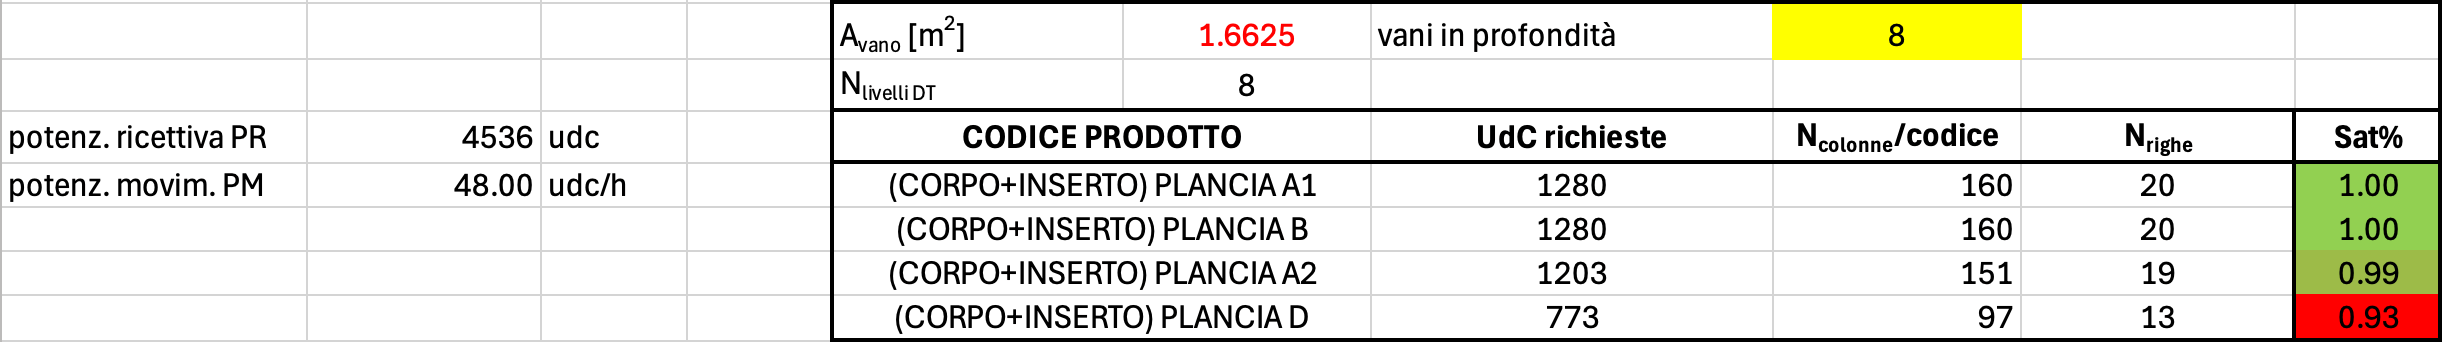
\includegraphics[width=\textwidth]{images/Dimensionamento statico magazzino drive-through BUFFER.png}
    \caption{Dimensionamento statico magazzino drive-through buffer}
    \label{fig: Dimensionamento statico magazzino drive-through BUFFER}
\end{figure}

\newpage
\paragraph{Dimensionamento dinamico}\mbox{}\\
Per il dimensionamento dinamico si sono calcolati i tempi di in e out, il numero di carrelli, la potenzialità di movimentazione effettiva. Le distanze orizzontali sono state calcolate dai punti di input/output ai baricentri del magazzino nel caso peggiore, ovvero più sfavorevole.
\begin{align}
    & H = \frac{N_{\text{liv,DT}} - 1}{2} \cdot h_{\text{vano}} \\
    & T_{\text{in}} = 2 \cdot T_{\text{f}} + \frac{L_{\text{in}}}{v_{\text{t,o,c}}} + \frac{L_{\text{in}}}{v_{\text{t,o,v}}} + \frac{H}{v_{\text{s,f,c}}} + \frac{H}{v_{\text{d,f,v}}} \\
    & T_{\text{out}} = 2 \cdot T_{\text{f}} + \frac{L_{\text{out}}}{v_{\text{t,o,c}}} + \frac{L_{\text{out}}}{v_{\text{t,o,v}}} + \frac{H}{v_{\text{s,f,v}}} + \frac{H}{v_{\text{d,f,c}}} \\
    & T_{\text{attr}} = T_{\text{in}} + T_{\text{out}} \\
    & N_{\text{carr}} = \text{ceil}\left(\frac{k \cdot \text{PM}_{\text{eff}} \cdot T_{\text{attr}}}{3600}\right) \\
    & \text{PM}_{\text{eff}} = \text{ceil}\left(\frac{N_{\text{carr}} \cdot 3600}{T_{\text{attr}}}\right) \\
    & N_{\text{van}} = N_{\text{liv,DT}} \cdot N_{\text{van,p}} \cdot N_{\text{rig,tot}} \\
    & A_{\text{mag,eff}} = \text{calcolata manualmente}
\end{align}

dove:
\begin{itemize}
    \item $N_{\text{liv,DT}}$ = numero livelli deposito temporaneo
    \item $h_{\text{vano}}$ = altezza vano
    \item $T_{\text{f}}$ = tempi fissi
    \item $L_{\text{in}}$ = lunghezza percorso in ingresso
    \item $L_{\text{out}}$ = lunghezza percorso in uscita
    \item $v_{\text{t,o,c}}$ = velocità traslazione orizzontale a carico
    \item $v_{\text{t,o,v}}$ = velocità traslazione orizzontale a vuoto
    \item $v_{\text{s,f,c}}$ = velocità salita forche a carico
    \item $v_{\text{d,f,v}}$ = velocità discesa forche a vuoto
    \item $v_{\text{s,f,v}}$ = velocità salita forche a vuoto
    \item $v_{\text{d,f,c}}$ = velocità discesa forche a carico
    \item $\text{PM}_{\text{eff}}$ = potenzialità movimentazione effettiva
    \item $N_{\text{carr}}$ = numero carrelli
    \item $N_{\text{van}}$ = numero vani totali
    \item $N_{\text{van,p}}$ = vani in profondità
    \item $N_{\text{rig,tot}}$ = righe totali
    \item $A_{\text{mag,eff}}$ = area magazzino effettiva
    \item $\text{PR}$ = potenzialità ricettiva
\end{itemize}

\newpage
Per quanto riguarda il magazzino è stato necessario rinunciare ad una forma ottimale e, di conseguenza ad un maggiore investimento, per ottenere un migliore sfruttamento degli spazi nel'’azienda. Il magazzino buffer assume quindi una forma a “L” con i blocchi in basso a destra adiacenti al muro, e quindi di tipologia drive in anziché drive through.

È possibile consultare tutti i calcoli effettuati per il dimensionamento del magazzino buffer nell'allegato "{{excelCompleto}}".
\newpage

\subsection{Dimensionamento magazzino PF}
\paragraph{Dimensionamento statico}\mbox{}\\
Il dimensionamento statico del magazzino prodotti finiti è stato effettuato considerando un vano di dimensioni 1900x950x950 mm, dimensioni che sono state successivamente utilizzate per il calcolo del numero di vani in altezza, in profondità, della linea e quelli totali.
Le formule utilizzate sono state le seguenti:
\begin{align}
    & N_\text{vani,alt} = \frac{S_ \text{max}}{h_\text{vano}} + 1 = 6 \\
    & N_\text{vani,prof} = 9 \text{ (definito arbitrariamente)} \\
    & N_\text{vani,lin} = N_\text{vani,alt} \cdot N_\text{vani,prof} = 54\\
    & h_\text{scaf} = N_\text{vani,alt} \cdot h_\text{vano} = 5.7 \text{ m}\\
    & p_\text{scaf} = N_\text{vani,prof} \cdot p_\text{vano} = 8.55 \text{ m}
\end{align}
dove:
\begin{itemize}
    \item $N_\text{vani,alt}$ = numero di vani in altezza
    \item $S_\text{max}$ = sollevamento massimo del carrello elevatore
    \item $h_\text{vano}$ = altezza del vano
    \item $N_\text{vani,prof}$ = numero di vani in profondità
    \item $N_\text{vani,lin}$ = numero di vani per linea
    \item $h_\text{scaf}$ = altezza dello scaffale
    \item $p_\text{scaf}$ = profondità dello scaffale
    \item $p_\text{vano}$ = profondità del vano
\end{itemize}
\vskip2em

\noindent
Successivamente, attraverso il numero di UdC di ciascuna plancia, è stato possibile definire il numero del modulo di base come:
\begin{equation}
    N_\text{MB} = \text{ceil}\left(\frac{N_\text{UDC}}{N_\text{vani,lin}}\right)
    \begin{cases}
        N_\text{MB,A1} = 21 \\
        N_\text{MB,A2} = 19 \\
        N_\text{MB,B} = 19 \\
        N_\text{MB,D} = 11
    \end{cases}
\end{equation}

\noindent
Solo a questo punto, si è potuto calcolare il numero dei vani totali come:
\begin{equation}
    N_\text{vani,tot} = N_\text{vani,lin} \cdot \sum_i N_{\text{MB},i} = 3780
\end{equation}

\newpage
Il dimensionamento statico procede quindi il calcolo delle aree e dell'inviluppo complessivo andando a definire le seguenti grandezze:
\begin{align}
    & N_\text{MB,tot} = \sum_i N_{\text{MB},i} = 70 \\
    & N_\text{aree} = 4 \text{( definito arbitrariamente)} \\
    & N_\text{MB,area} = \text{ceil}\left(\frac{N_\text{MB,tot}}{N_\text{aree}}\right) = 18 \\
    & L_\text{area} = N_\text{MB,area} \cdot L_\text{vano} = 18 \cdot 1.9 = 34.2 \text{ m} \\
    & L_\text{corr,princ} = 6 \text{ m (definito arbitrariamente)} \\
    & L_\text{corr,sec} = 3.2 \text{ m (definito arbitrariamente)}
\end{align}
\noindent
dove:
\begin{itemize}
    \item $N_\text{MB,tot}$ = numero totale di moduli base
    \item $N_\text{aree}$ = numero di aree
    \item $N_\text{MB,area}$ = numero di moduli base per area
    \item $L_\text{area}$ = lunghezza dell'area
    \item $L_\text{vano}$ = lunghezza del vano
    \item $L_\text{corr,princ}$ = lunghezza del corridoio principale
    \item $L_\text{corr,sec}$ = lunghezza del corridoio secondario
\end{itemize}
\vskip2em

\noindent
A questo punto, è possibile finalmente calcolare le dimensioni effettive dell'inviluppo del magazzino prodotti finiti:
\begin{align}
    & U_\text{eff} = 2 \cdot L_\text{area} + L_\text{corr,princ} = 2 \cdot 34.2 + 6 = 74.4 \text{ m} \\
    & V_\text{eff} = 2 \cdot p_\text{scaf} + L_\text{corr,princ} + 2 \cdot L_\text{corr,sec} = 2 \cdot 8.55 + 6 + 2 \cdot 3.2 = 32.3 \text{ m} \\
    & A_\text{eff} = U_\text{eff} \cdot V_\text{eff} = 74.4 \cdot 32.3 = 2403 \text{ m}^2
\end{align}

\begin{figure}[H]
    \centering
    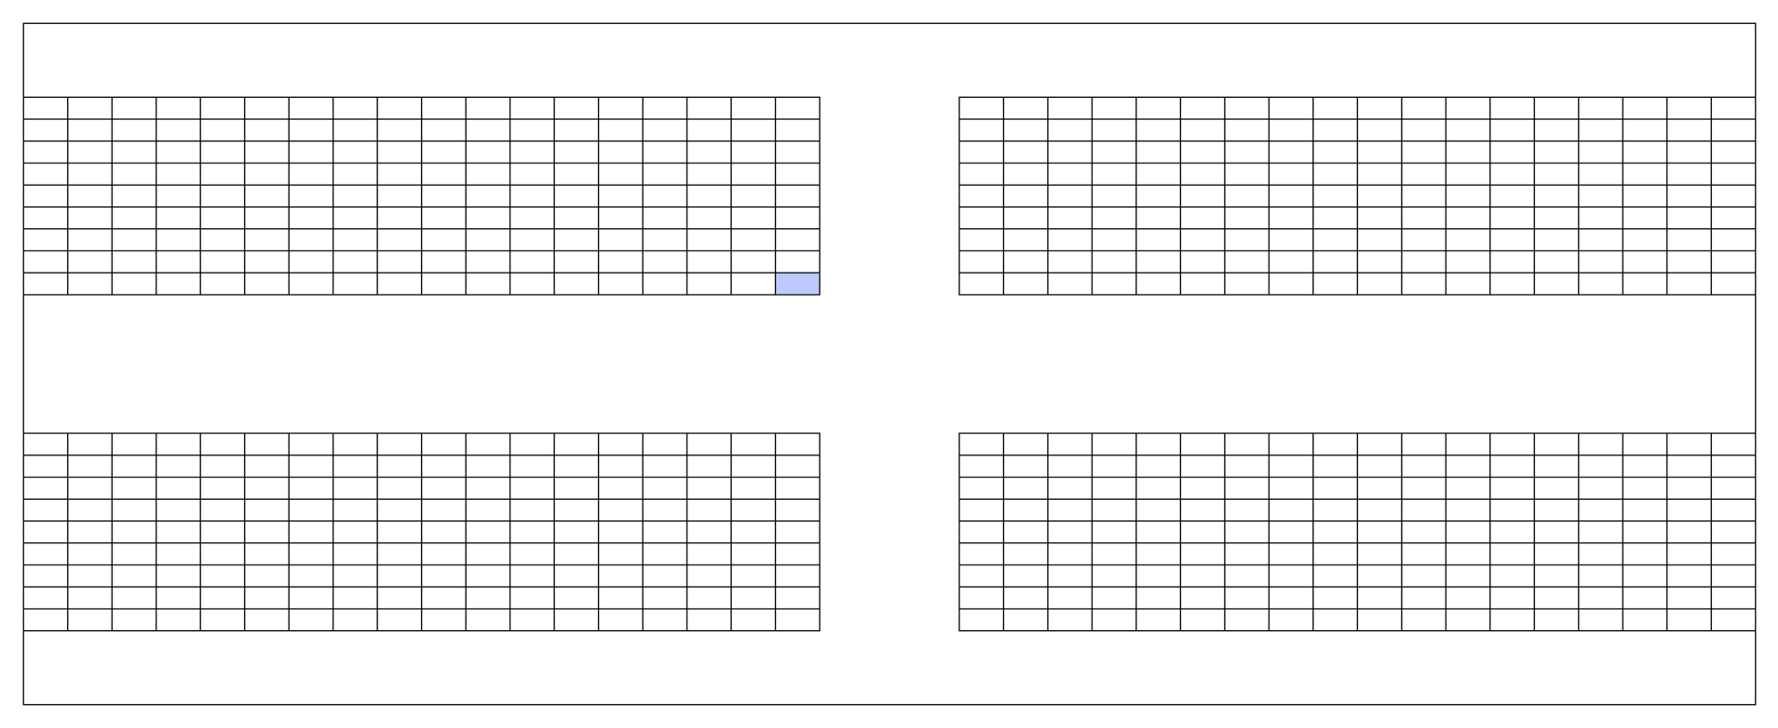
\includegraphics[width=\textwidth]{images/Dimensionamento statico magazzino PF.png}
    \caption{Dimensionamento statico del magazzino prodotti finiti}
    \label{fig: Dimensionamento statico del magazzino prodotti finiti}
\end{figure}
\newpage

\paragraph{Dimensionamento dinamico}\mbox{}\\
Il dimensionamento dinamico è stato effettuato considerando alcune grandezze relative al carrello elevatore e altre più generali come:
\begin{align*}
    & v_\text{tr,vuo} = 2.78 \text{ m/s} \\
    & v_\text{tr,car} = 2.22 \text{ m/s} \\
    & v_\text{sol,for,vuo} = 0.36 \text{ m/s} \\
    & v_\text{sol,for,car} = 0.17 \text{ m/s} \\
    & v_\text{dis,for,vuo} = 0.47 \text{ m/s} \\
    & v_\text{dis,for,car} = 0.45 \text{ m/s} \\
    & k = 1.2 \\
    & N_\text{gg} = 4 \\
    & N_\text{ore} = 14.33 \text{ h} \\ 
    & \text{UdC}_\text{mov} = 3050
\end{align*}
\noindent
dove:
\begin{itemize}
    \item $v_\text{tr,vuo}$ = velocità di traslazione a vuoto
    \item $v_\text{tr,car}$ = velocità di traslazione a carico
    \item $v_\text{sol,for,vuo}$ = velocità di sollevamento forche a vuoto
    \item $v_\text{sol,for,car}$ = velocità di sollevamento forche a carico
    \item $v_\text{dis,for,vuo}$ = velocità di discesa forche a vuoto
    \item $v_\text{dis,for,car}$ = velocità di discesa forche a carico
    \item $k$ = coefficiente di utilizzazione
    \item $N_\text{gg}$ = numero di giorni lavorativi
    \item $N_\text{ore}$ = numero di ore lavorative giornaliere ottimizzate
    \item $\text{UdC}_\text{mov}$ = unità di carico movimentate
\end{itemize}
\vskip2em

\noindent
Al fine di calcolare l'importa, è possibile prima determinare il percorso sul piano e in altezza del carrello elevatore come:
\begin{align}
    & p_\text{piano} = L_\text{corr,sec} + p_\text{scaf} + \frac{L_\text{corr,princ}}{2} + \frac{L_\text{corr,princ}}{2} + \frac{L_\text{area}}{2} + \frac{L_\text{corr,princ}}{2} = 38.05 \text{ m} \\
    & p_\text{altezza} = \frac{N_\text{vani,alt} - 1}{2} \cdot h_\text{vano} = 2.38 \text{ m}
\end{align}

\noindent
A questo punto, è possibile definire la potenzialità di movimentazione in entrata e in uscita come:
\begin{align}
    & \text{PM}_\text{in} = \text{ceil}\left(\frac{\text{UdC}_\text{mov}}{N_\text{gg} \cdot N_\text{ore}}\right) = 54 \text{ UdC/h} \\
    & \text{PM}_\text{out} = \text{ceil}\left(\frac{\text{max}(N_{\text{UdC},i})}{N_\text{ore}}\right) = 77 \text{ UdC/h}
\end{align}

\newpage
\noindent
Inoltre, è possibile calcolare il tempo ciclo in entrata e in uscita come:
\begin{align}
    & \text{TC}_\text{in} = 2 \cdot T_\text{fis} + \frac{p_\text{piano}}{v_\text{tr,car}} + \frac{p_\text{altezza}}{v_\text{sol,for,car}} + \frac{p_\text{altezza}}{v_\text{dis,for,vuo}} + \frac{p_\text{piano}}{v_\text{tr,vuo}} = 169.84 \text{ s} \\
    & \text{TC}_\text{out} = 2 \cdot T_\text{fis} + \frac{p_\text{piano}}{v_\text{tr,vuo}} + \frac{p_\text{altezza}}{v_\text{sol,for,vuo}} + \frac{p_\text{altezza}}{v_\text{dis,for,car}} + \frac{p_\text{piano}}{v_\text{tr,car}} = 162.70 \text{ s}
\end{align}

\noindent
Da questi valori è possibile eseguire una media pesata con le potenzialità di movimentazione in entrata e in uscita per ottenere il tempo di attraversamento medio:
\begin{equation}
    T_\text{attr} = \frac{\text{PM}_\text{in} \cdot \text{TC}_\text{in} + \text{PM}_\text{out} \cdot \text{TC}_\text{out}}{\text{PM}_\text{in} + \text{PM}_\text{out}} = 165.64 \text{ s}
\end{equation}

\noindent
Con le grandezze precedenti, è possibile calcolare il numero di carrelli necessari per soddisfare la potenzialità di movimentazione richiesta:
\begin{align}
    & N_\text{carr,teo,in} = k \cdot \text{PM}_\text{in} \cdot \text{TC}_\text{in} = 3.06 \\
    & N_\text{carr,teo,out} = k \cdot \text{PM}_\text{out} \cdot \text{TC}_\text{out} = 4.18 \\
    & N_\text{carr,eff} = \text{ceil}\left(N_\text{carr,teo,in} + N_\text{carr,teo,out}\right) = 8
\end{align}

\noindent
È possibile concludere il dimensionamento dinamico calcolando l'impronta del magazzino prodotti finiti come:
\begin{equation}
    \text{CUS}_\text{eff} = \frac{\sum_i N_{\text{UdC},i}}{A_\text{eff}} = 1.52
\end{equation}

\begin{figure}[H]
    \centering
    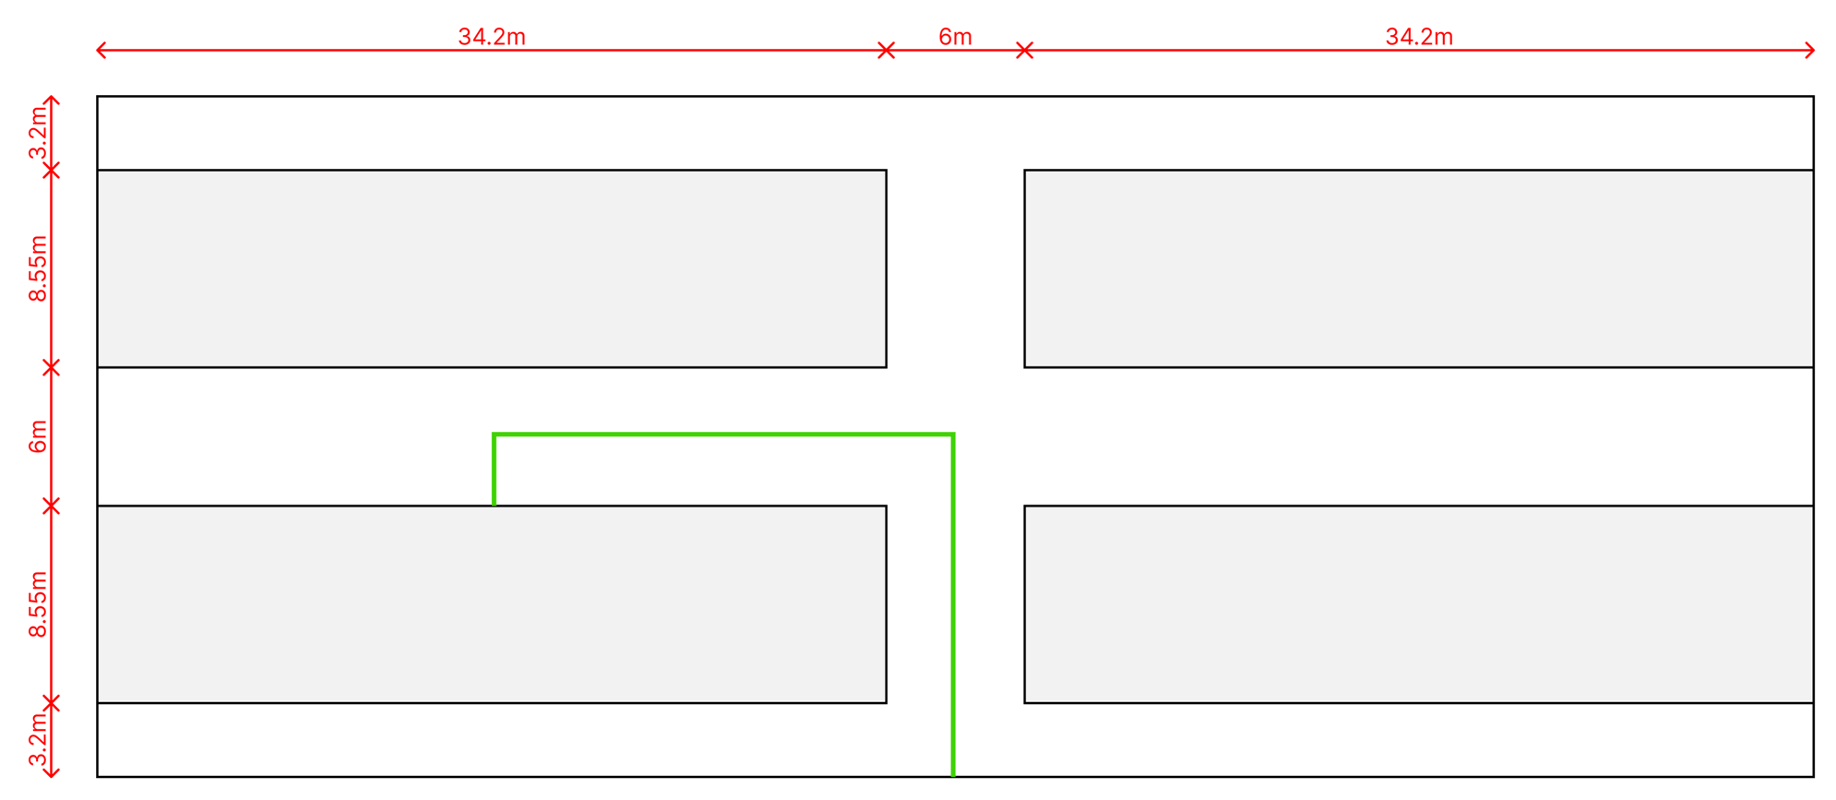
\includegraphics[width=\textwidth]{images/Dimensionamento dinamico magazzino PF (vista in pianta).png}
    \caption{Dimensionamento dinamico del magazzino prodotti finiti (vista in pianta)}
    \label{fig: Dimensionamento dinamico del magazzino prodotti finiti (vista in pianta)}
\end{figure}

\begin{figure}[H]
    \centering
    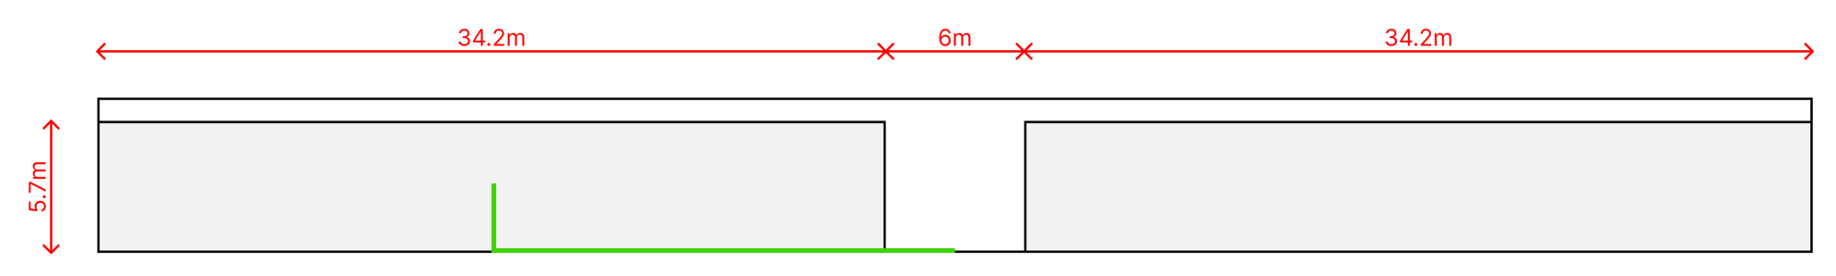
\includegraphics[width=\textwidth]{images/Dimensionamento dinamico magazzino PF (vista frontale).png}
    \caption{Dimensionamento dinamico del magazzino prodotti finiti (vista frontale)}
    \label{fig: Dimensionamento dinamico del magazzino prodotti finiti (vista frontale)}
\end{figure}

\noindent
Per consultare tutti i calcoli effettuati per il dimensionamento del magazzino prodotti finiti, è possibile fare riferimento all'allegato "{{excelCompleto}}".
\newpage

\subsection{Analisi ABC}
Il dimensionamento ABC è stato effettuato sui parametri di giacenza media e indice di rotazione. I calcoli che sono stati eseguiti riguardano il magazzino materie prime in quanto presenta molti più articoli e codici rispetto al magazzino buffer e prodotti finiti, per i quali l'analisi ABC sarebbe risultata superflua.
Per l'analisi ABC si è effettuato il calcolo della percentuale per ogni indice di rotazione sul totale (somma dei singoli indici di rotazione degli articoli a magazzino materie prime) e si è proceduto con la determinazione della percentuale cumulata. Gli stessi calcoli sono stati effettuati considerando al posto dell'indice di rotazione i valori di giacenza media.
Grazie a ciò è stato possibile costruire un grafico per l'indice di rotazione e la giacenza media, i valori di cumulata rientranti nell'80\% appartengono alla classe A (quella più ad alta movimentazione e che richiede la priorità maggiore), quelli rientranti dall'80 al 95\% rientrano nella classe B e i restanti nella classe C.

\begin{figure}[H]
    \centering
    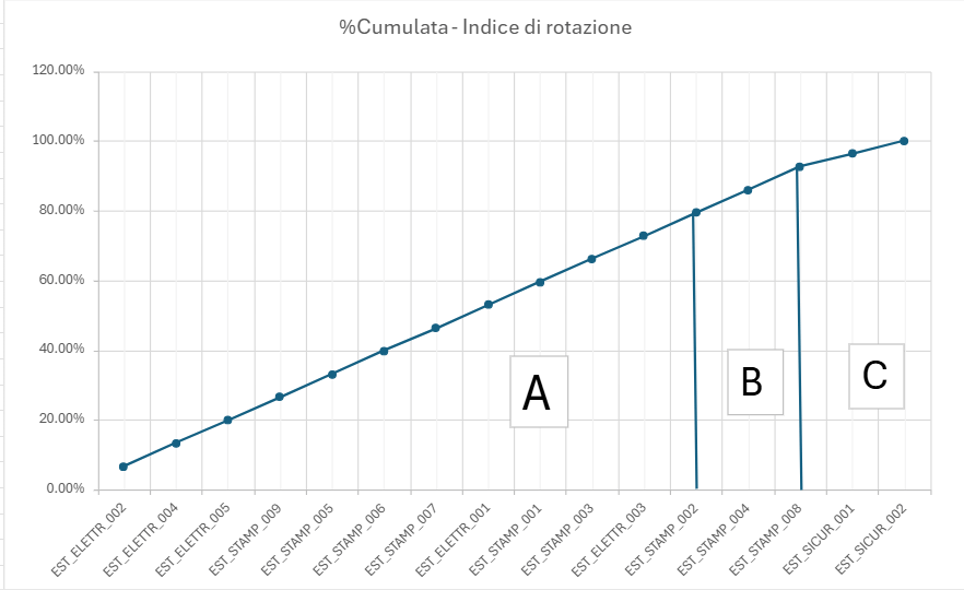
\includegraphics[width=\textwidth]{images/Analisi ABC.png}
    \caption{Analisi ABC}
    \label{fig: Analisi ABC}
\end{figure}

\noindent
È possibile consultare l'analisi ABC completa nell'allegato "{{excelCompleto}}".
\newpage

\subsection{Dimensionamento area di picking}
\subsubsection{Calcoli relativi alla domanda}
Per determinare il layout dell'area di picking e la procedura di preparazione kit, si parte dalla richiesta di kit proveniente dall'area produttiva.
Come base numerica di riferimento, è stato considerato il fabbisogno mensile, da cui è stato successivamente calcolato il numero di kit necessari a soddisfare la domanda giornaliera per tutti e quattro i prodotti della zona di assemblaggio, tenendo conto degli indici di utilizzo di ciascun componente indicati nelle rispettive distinte base. 
\vskip4em

\subsubsection{Produzione kit}
Dopo aver individuato i fabbisogni per ciascun prodotto (A1, A2, B, D), è stato calcolato il TT di produzione dei kit, ovvero il ritmo necessario per soddisfare la domanda. Considerando un tempo ciclo di 2,5 minuti, il valore è stato suddiviso per il numero di linee produttive assegnate a ciascun prodotto. 
Ad esempio, per il prodotto A1 si è ottenuto il seguente risultato:
\begin{equation}
    \text{TT}_{A1} = \frac{2,5}{4} = 0,625 \text{ min}
\end{equation}
\noindent
Lo stesso procedimento è stato applicato per gli altri tre prodotti.
\vskip4em

\subsubsection{Distribuzione e tempistiche}
Per definire i ritmi di distribuzione nell'area produttiva, si è partiti dalla scelta del carrello elevatore "BTSTAXIO” (le cui specifiche possono essere consultate su {{elevatoreBTSTAXIO}}), individuando successivamente nella documentazione tecnica la velocità massima raggiungibile, pari a 15 km/h. A partire da questa informazione, e utilizzando il file CAD dell'impianto, sono state calcolate le distanze medie percorse dal carrello per il rifornimento delle tre principali zone di assemblaggio: A1, A2, e B + D. Il tragitto medio stimato risulta pari a 230 metri.

Successivamente, è stato definito un metodo di scarico dei vagoni basato sull'utilizzo di pallet con ruote. Questo ha permesso di stimare un tempo di sosta medio per linea pari a 10 secondi, necessario unicamente per spingere il pallet fuori dal vagone. Moltiplicando questo tempo per il numero di linee assegnate a ciascun prodotto, è stato possibile determinare il tempo totale di attraversamento per ciascuna macro-area. Ad esempio, per l’area B + D, il tempo complessivo risulta pari a:
\begin{equation}
    T_\text{BD} = \frac{s}{v} + N_\text{tot,lin} \cdot 10 = 0.029 \, \text{h}
\end{equation}

dove:
\begin{itemize}
    \item $T_\text{BD}$ = tempo per l'area B + D
    \item $s$ = spazio percorso (230 m)
    \item $v$ = velocità del carrello (15 km/h)
    \item $N_\text{tot,lin}$ = numero totale di linee (in totale 5, 3 per il prodotto B e 2 per il prodotto D)
\end{itemize}
\newpage

Una volta calcolati i tempi di attraversamento per ciascuna area, si è passati a stimare il tempo di produzione che una singola consegna era in grado di saturare. Considerando una capacità di trasporto di 16 contenitori Odette per vagone (disposti 4x4), si ottiene un totale di 64 kit per viaggio.
Nel caso del prodotto A1, il tempo di saturazione è stato calcolato come:
\begin{equation}
    T = \frac{N_\text{kit}}{\text{TC} \cdot N_{\text{lin},A1} } = \frac{64}{2{,}5 \times 0{,}625} = 40 \, \text{min}
\end{equation}
dove:
\begin{itemize}
    \item $N_\text{kit}$ = numero di kit totali
    \item $N_{\text{lin},A1}$ = numero di linee assegnate al prodotto A1
\end{itemize}

\noindent
Questo significa che 64 kit sono sufficienti per tenere occupata una linea A1 per 40 minuti. Partendo da questo tempo di saturazione, si è considerato che tutti i kit necessari in quel periodo dovessero essere prodotti e distribuiti nelle varie postazioni prima della scadenza di tale intervallo, per evitare tempi di fermo.

Per il prodotto A1, questo equivale a dover produrre, in un tempo utile pari a 35,2 minuti (cioè 40 minuti meno il tempo di distribuzione), le seguenti quantità:
\begin{equation}
    N_\text{kit,tot,A1} = N_\text{kit,A1} \cdot N_\text{lin,A1} = 64 \cdot 3 = 192 \, \text{kit}
\end{equation}
dove:
\begin{itemize}
    \item $N_\text{kit,tot,A1}$ = numero totale di kit per il prodotto A1
    \item $N_\text{kit,A1}$ = numero di kit per linea del prodotto A1
    \item $N_\text{lin,A1}$ = numero di linee assegnate al prodotto A1
\end{itemize}

\noindent
Il ritmo produttivo medio risulta quindi pari a:
\begin{equation}
    R_\text{kit,A1} = \frac{T_u}{N_\text{kit,tot,A1}} = \frac{35{,}2}{192} \approx 11 \, \text{s/kit}
\end{equation}
dove:
\begin{itemize}
    \item $R_\text{kit,A1}$ = ritmo produttivo medio per il prodotto A1
    \item $T_u$ = tempo utile per la produzione (35,2 minuti)
    \item $N_\text{kit,tot,A1}$ = numero totale di kit per il prodotto A1
\end{itemize}

Considerando un totale di 6 operatori, la produzione individuale corrisponde a circa 1 kit ogni 1,1 minuti per operatore.

\begin{figure}[H]
    \centering
    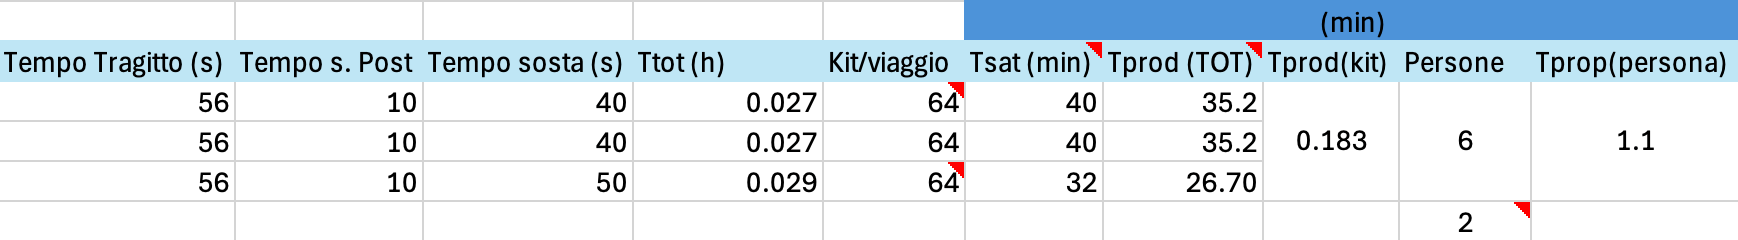
\includegraphics[width=\textwidth]{images/Picking.png}
    \caption{Area di picking}
    \label{fig: Area di picking}
\end{figure}

Producendo in ordine i kit B e D in soli 12 minuti si può far partire il trenino che in 1,62 minuti riesce a distribuire e tornare nell'area di picking per essere ricaricato e per andare a rifornire le altre aree.

Tutti i calcoli sono disponibili nell'apposita sezinoe dell'allegato "{{excelCompleto}}" mentre il layout dell'area di picking è disponibile nell'allegato "{{areaPicking}}".

\newpage

\subsection{Dimensionamento banchine carico/scarico}
\subsubsection{Calcoli relativi a camion}
Per il calcolo del numero di camion in arrivo, si determina innanzitutto il numero di udc in arrivo per ogni categoria (sicurezza, elettrica e stampati) come somma delle UdC appartenenti alla stessa famiglia di prodotti.
Dopodichè si calcola il numero di udc per ogni camion cercando di saturarlo il più possibile, senza eccedere il limite di peso del rimorchio.
Il rimorchio scelto è un rimorchio telonato, le cui specifiche possono essere reperite sul sito ufficiale DSV \cite{dsv_trailer}.

\vskip1cm
\noindent
Si determina quindi il numero di camion come:
\begin{equation}
    N_\text{cam} = \text{ceiling}\left(\frac{N_\text{UdC}}{N_\text{UdC/cam}}\right)
    \qquad
    \begin{cases}
        N_\text{cam} = \text{numero di camion} \\
        N_\text{UdC} = \text{numero di UdC} \\
        N_\text{UdC/cam} = \text{numero di UdC per camion}
    \end{cases}
\end{equation}

\noindent
Si calcolano, infine, il tempo totale di scarico e il numero di banchine teorico per ogni categoria come:
\begin{align}
    & T_\text{tot} = N_\text{cam} \cdot t_\text{sc} \\
    & N_\text{banch,th} = \frac{T_\text{tot}}{T_\text{tur}}
\end{align}

\noindent
dove:
\begin{itemize}
    \item $T_\text{tot}$ = tempo totale di scarico
    \item $t_\text{sc}$ = tempo di scarico per camion
    \item $N_\text{banch,th}$ = numero di banchine teorico
    \item $T_\text{tot}$ = tempo totale disponibile giornaliero
    \item $T_\text{tur}$ = tempo turno giornaliero
\end{itemize}

Per determinare il numero effettivo di banchine, si deve prima determinare la sovrapposizione in termini di consegne peggiore che si è determinata avvenire tra gli stampati e le ODETTE di sicurezza, si calcola poi il numero di banchine effettivo come arrotondamento della somma delle banchine teoriche per queste due categorie.
\subsubsection{Camion e banchine in entrata}
Per il calcolo dei camion in entrata si segue il procedimento descritto sopra, tenendo conto del fatto che le consegne avvengono ogni 4 giorni per ogni codice.
Per il calcolo delle banchine, in questo caso, si sceglie di arrotondare al numero di banchine teorico maggiore, in quanto corrispondente al maggior numero di UdC movimentate in uscita in un giorno.
\subsubsection{Area di ricevimento}
Per il calcolo delle aree di ricevimento e controllo merce si è mantenuto costante il lato dell'area di ricevimento affacciato alle banchine di carico, di 4 metri, corrispondenti a 3,2 m di udc più 0,8 m di corridoio d'ispezione.
Le aree determinate sono basate sulle necessità di ricezione del giorno con più arrivi, e sono le seguenti: due aree di 40 $m^2$, un'area di 24 $m^2$ e tre di 45 $m^2$, rispettivamente destinate a cupolotti/inserti plancia, ODETTE e corpi plancia.
È possibile consultare il layout dell'area di ricevimento nell'allegato "{{areaRicezione}}".
\newpage

\subsection{Calcolo trasporti interni}
Per il calcolo dei trasporti interni sono stati calcolati i seguenti parametri:
\begin{align}
    & T_\text{spo} = 2 \times \left( \frac{D}{V_\text{tra}} + T_\text{fissi} \right) \\
    & T_\text{tot, men} = T_\text{spo} \times M_\text{men} \\
    & N_\text{mezzi} = \frac{T_\text{tot, men}}{0.8 \times T_\text{disp}}
\end{align}

\noindent
dove:
\begin{itemize}
    \item $T_\text{spo}$ = tempo di spostamento
    \item $D$ = distanza tra i reparti
    \item $V_\text{tra}$ = velocità di traslazione del carrello
    \item $T_\text{fissi}$ = tempi fissi per operazioni di carico/scarico
    \item $T_\text{tot, men}$ = tempo totale mensile
    \item $T_\text{spo}$ = tempo di spostamento
    \item $M_\text{men}$ = movimentazione mensile
    \item $N_\text{mezzi}$ = numero di mezzi necessari
    \item $T_\text{disp}$ = tempo disponibile mensile
\end{itemize}
\vskip4em

Per il calcolo del numero effettivo di carrelli si è preso il numero teorico di carrelli precedentemente calcolato e lo si è moltiplicato per un fattore correttivo basato sulla durata della batteria dichiarata dal fornitore che si è così calcolata:
\begin{equation}
    D_\text{batt} = \frac{C_\text{nom}}{C_\text{cons} \times 1000/V_\text{batt}} = 9.35 \text{ h}
\end{equation}

\noindent
dove:
\begin{itemize}
    \item $D_\text{batt}$ = durata della batteria
    \item $C_\text{nom}$ = capacità nominale della batteria (in Ah)
    \item $C_\text{cons}$ = consumo energetico del carrello (in kWh/h)
    \item $V_\text{batt}$ = tensione della batteria (in V)
\end{itemize}
\vskip2em

\noindent
Il coefficiente correttivo è stato calcolato come:
\begin{equation}
    c = \frac{h_\text{giorno}}{D_\text{batt}} = \frac{14}{9.35} = 1.53
\end{equation}
\noindent
Il numero teorico di carrelli è stato quindi moltiplicato per questo coefficiente, ottenendo il numero effettivo di carrelli necessari:
\begin{equation}
    N_\text{carr,eff} = N_\text{carr,teo} \cdot c = 44 \cdot 1.53 \approx 68
\end{equation}
\newpage


\section{Personale e aree accessorie}
\subsection{Determinazione del numero di addetti diretti e indiretti}
Per calcolare il numero di addetti alla produzione è stato calcolato considerando un'addetto per ogni postazione di saldatura e assemblaggio, per due turni.

Per calcolare il numero di addetti alla logistica è stato considerato un addetto per ogni carrello teorico, uno per il pallettizattore, uno per ogni postazione del picking più uno per il carico delle odette sul trenino nell'area di picking.

Il numero di dipendenti indiretti è stato valutato come il 20\% del totale dei dipendenti diretti.
\vskip4em

\subsection{Dimensionamento impianto di aria compressa}
L'analisi dell'impianto d'aria compressa ha interessato la zona di saldatura e la zona di assemblaggio. La decisione è ricaduta in ambe le zone su una configurazione ad anello, un anello unico per la zona di saldatura e quattro anelli distinti per la zona di assemblaggio.
Il fabbisogno degli utilizzatori nelle due aree era già fornito assieme agli altri parametri presenti in tabella:

\begin{table}[H]
    \centering
    \renewcommand{\arraystretch}{1.5}
    \resizebox{\textwidth}{!}{
    \begin{tabular}{|c|c|c|c|c|c|}
        \hline
        \textbf{} & \textbf{} & \textbf{CONSUMO ARIA LIBERA} & \textbf{FT (base)} & \textbf{FL} & \textbf{PRESSIONE} \\
        & & {[}m\textsuperscript{3}/h{]} & \% & \% & {[}bar{]} \\
        \hline
        \multirow{2}{*}{\textbf{SALDATURA}} & Molatrice & 90 & 20 & 40 & 6,5 \\
        \cline{2-6}
         & Perforatrice & 120 & 15 & 70 & 6,5 \\
        \hline
        \multirow{2}{*}{\textbf{ASSEMBLAGGIO}} & Avvitatore & 70 & 25 & 30 & 6,5 \\
        \cline{2-6}
         & Rivettatrice & 30 & 5 & 15 & 6,5 \\
        \hline
    \end{tabular}}
    \caption{Consumo aria compressa per saldatura e assemblaggio}
    \label{tab:consumo_aria}
\end{table}

\noindent
Il parametro FT è stato moltiplicato per un fattore K conferito per ogni utilizzatore, ottenendo così il fabbisogno teorico per utilizzatore, che nel nostro caso è pari a 1.7416.
\vskip4em

\subsubsection*{Step 1}
Abbiamo calcolato il fabbisogno di AC (Aria compressa) necessaria per ogni parte del circuito mediante la formula:
\begin{equation}
    \text{AC} = (1+\text{SF}) \cdot \sum _{i=1}^{n}  \frac{A_i \cdot B_i \cdot  C_i}{100}
\end{equation}
\noindent
dove:
\begin{itemize}
    \item $\text{SF}$ = fattore di sicurezza (circa 10\%-30\%)
    \item $A_i$ = numero di strumenti
    \item $B_i$ = fattore di carico (ottenuto moltiplicando il FT per il FL)
    \item $C_i$ = consumo aria libera [m\textsuperscript{3}/h]
\end{itemize}

\noindent
Considerando il fattore di sicurezza SF solo nel computo totale (TOT in tabella) e direttamente nel calcolo delle perdite di pressione dei vari rami (PD in tabella step 3).
\begin{figure}[H]
    \centering
    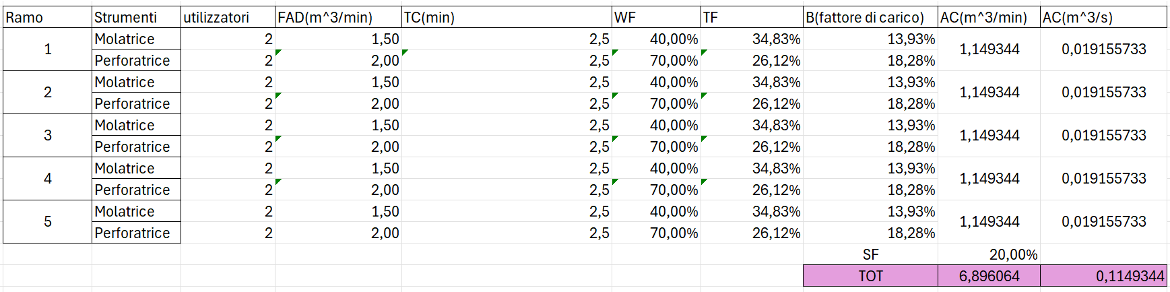
\includegraphics[width=\textwidth]{images/Step 1 aria compressa.png}
    \caption{Step 1 aria compressa}
    \label{fig: Step 1 aria compressa}
\end{figure}

\noindent
Si assumono necessari una molatrice e una perforatrice per ogni postazione, dunque il numero di utilizzatori per ogni tipologia di strumento equivale al numero di postazioni alimentate dal ramo i-esimo (2 postazioni per ogni ramo).
Mentre il fattore di carico B è stato calcolato mediante la moltiplicazione del fattore tempo con il fattore di lavoro.
\vskip4em

\subsubsection*{Step 2}
Abbiamo analizzato le caratteristiche geometriche del sistema come la lunghezza L e il diametro della condotta (sono stati utilizzati dei diametri standardizzati).
\begin{figure}[H]
    \centering
    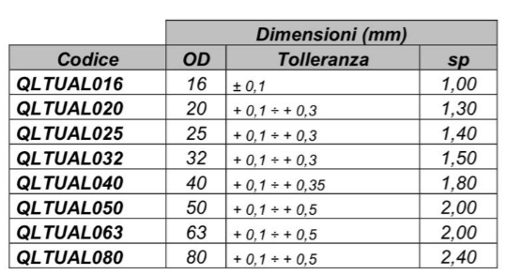
\includegraphics[width=0.5\textwidth]{images/Step 2 aria compressa.png}
    \caption{Step 2 aria compressa}
    \label{fig: Step 2 aria compressa}
\end{figure}

\noindent
La valutazione dei diametri è stata effettuata seguendo questi passaggi. In primo luogo, è stato calcolato l'area necessaria in base alla portata di aria compressa richiesta. Da questa area è stato determinato il diametro interno della conduttura (D). Infine, è stata verificata la velocità effettiva dell'aria (V\textsubscript{eff}).

Il valore di velocità dell'aria è stato assunto come standard. Dopo aver calcolato il diametro interno effettivo, è stata verificata la velocità dell'aria che deve rispettare il seguente vincolo:
\begin{equation}
    6\,\text{m/s} < V_\text{eff} < 10\,\text{m/s}
\end{equation}
\vskip4em

\subsubsection*{Step 3}
Infine, nell'ultimo step abbiamo calcolato le perdite di carico nelle varie posizioni del sistema per poter analizzare il punto con la maggiore perdita di pressione e dimensionare il generatore di aria compressa.
Per il calcolo delle perdite di carico, come primo passo è necessario determinare la quantità di giunti e valvole presenti nelle varie zone dell'impianto.
Successivamente, si valuta la perdita di carico equivalente in metri (dalla tabella), in base al diametro della condotta.
\begin{figure}[H]
    \centering
    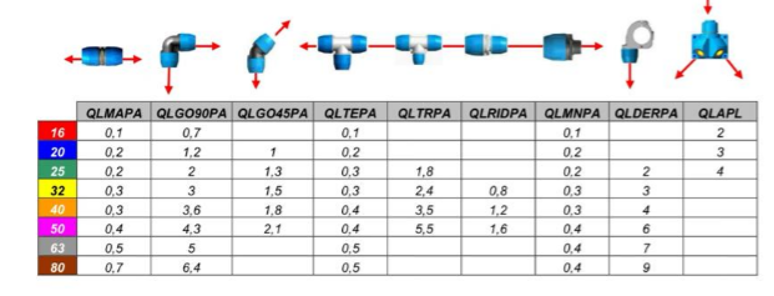
\includegraphics[width=0.8\textwidth]{images/Step 3 aria compressa.png}
    \caption{Step 3 aria compressa}
    \label{fig: Step 3 aria compressa}
\end{figure}

Per la determinazione delle valvole è necessario considerare i punti più sensibili, come l'inizio e l'uscita dell'anello, dove sono presenti rispettivamente 3 e 2 valvole, e le due estremità dei rami, dove è presente una valvola per estremità.
I giunti dritti sono stati considerati come punti di collegamento tra i vari tratti di tubi, ciascuno di lunghezza massima di 6 metri.
I tubi flessibili, che permettono all'aria compressa di raggiungere l'utilizzatore, sono stati considerati come tubi rigidi per semplificare il calcolo. La lunghezza del tubo è stata determinata considerando un'altezza della conduttura di 9 metri, poiché il punto più alto presente nei magazzini è di 7 metri, a cui sono stati aggiunti 2 metri di margine per eventuali incidenti.
È stata analizzata la somma delle perdite nel loop-ring, nella condotta dal generatore al loop-ring e nei singoli rami per identificare il punto con la perdita di carico maggiore.
Infine, per il calcolo della pressione necessaria, è stata sommata la compression ratio con la perdita massima e un margine di 1,5 bar.
\vskip4em

\subsubsection*{Step 4}
Gli stessi calcoli sono stati effettuati per gli altri quattro anelli dell'assemblaggio e infine abbiamo confrontato quale dei 5 anelli complessivi presentasse la perdita di carico maggiore, al fine di dimensionare il generatore complessivo dell'impianto.
È risultato che la pressione maggiore è richiesta dall'anello della zona di saldatura, pari a:
\begin{equation}
    P_\text{max} = 8,5084\,\text{bar}
\end{equation}
\vskip4em

\noindent
È possibile consultare i calcoli nell'allegato "{{ariaCompressaAssemblaggio}}".

\newpage

\section{Sicurezza}
\subsection{Dimensionamento uscite di sicurezza anti incendio}
Attraverso la formula:
\begin{equation}
    q_f = \frac{g_i \cdot H_{u,i} \cdot  m_i \cdot \psi_i}{A_f}
\end{equation}
si è determinato il carico specifico d'incendio delle varie aree di stoccaggio, tutte contenenti materiali infiammabili (polipropilene, \(H_u = 43\,\text{MJ/kg}\)) e tutte conseguentemente classificate come a rischio d'incendio medio e con necessità di uscite di sicurezza con classe REI di 60 per MP, e 120 per PF e buffer.

Le aree produttive di saldatura e assemblaggio, oltre alle aree accessorie, visto il contenuto ridotto di materiali infiammabili, sono state classificate a rischio d'incendio basso.

Segue da quanto detto sopra che le aree di immagazzinamento vanno isolate dal resto dello stabilimento e necessitano di uscite di sicurezza raggiungibili al massimo da una distanza di 45 m, mentre le restanti parti dello stabilimento necessitano di uscite di sicurezza raggiungibili al massimo da una distanza di 60 m, oppure di scale antincendio per le sezioni dell'edificio composte da più di un piano.

Per garantire un'uscita verso l'esterno che sia sicura in caso di incendio è stato previsto un marciapiede perimetrale in tutto lo stabilimento con larghezza 1,2 m.
\newpage

\subsection{Applicazione del metodo di Niosh}
\subsubsection{Saldatura}
Per la saldatura sono stati considerati tutti i componenti con peso superiore a 3 kg.

Il metodo utilizzato fa riferimento ad una situazione sequenziale, con un numero di atti al minuto pari a \(1/T_\text{ciclo}\) e i pezzi presi e immessi tutti nel ripiano inferiore di ogni UdC per un calcolo conservativo.

La procedura è la seguente:
\begin{align*}
    \text{PR} &= CP \times \text{FATTORI CORRETTIVI} \\
    \text{IS} &= \frac{\text{PR}}{\text{P}_\text{eff}} \\
    \text{PR}_\text{max} &= \text{CP} \times \text{FAT. CORR. con FF}_\text{max} \\
    \text{IS}_\text{max} &= \frac{\text{PR}_\text{max}}{\text{P}_\text{eff}} \\
\end{align*}

Successivamente si ordina in ordine decrescente \(\text{IS}_\text{max}\) e si calcola il coefficiente \(k\) come:
\begin{equation}
    k = \frac{\sum_{n-1} \text{IS}_{\text{max}, i} \times \text{FT}_i}{\text{IS}_{\text{max}, 1}}
\end{equation}

\noindent
Infine si calcola l'ISCS come:
\begin{equation}
    \text{ISCS} = \text{IS}_1 - (\text{IS}_{\text{max}, 1} - \text{IS}_1) \times k
\end{equation}

\noindent
Considerando che il valore di ISCS risulta essere 1.25, si conclude che il rischio è in fascia di attenzione.
\vskip4em


\subsubsection{Picking (carico)}
Per il calcolo dell'ISCS nel picking (solo nella fase di carico) la procedura è la stessa indicata sopra, si ottiene un ISCS di 1.49, corrispondente al livello di rischio.

In precedenza si era ottenuto un valore superiore a 5, che richiedeva un intervento immediato di prevenzione, motivo per cui abbiamo aggiunto un ulteriore operatore per ridurre la frequenza degli atti/min.

\vskip2em
\noindent
È possibile consultare i calcoli nell'allegato "{{excelCompleto}}".
\newpage


\section{Punti facoltativi}
\subsection{Value Stream Map}
Per ogni categoria di prodotto sono stati riportati:
\begin{itemize}
    \item Frequenza di arrivo
    \item \(\#\) pezzi/mese
    \item \(\#\) pezzi a magazzino MP in un ciclo di riordino
    \item \(T_{\text{ciclo}}\), \(T_{\text{setup}}\), dimensione lotto, \(T_{\text{disponibile}}\), UE di saldatura e assemblaggio
    \item Giacenza media per ciascun magazzino
    \item Tempi effettivi di lavorazione
    \item \(\#\) pezzi a magazzino buffer in un ciclo di riordino
    \item \(\#\) pezzi a magazzino PF in un ciclo di riordino
    \item Frequenza delle consegne da magazzino PF
\end{itemize}

\noindent
Di seguito, è possibile vedere un esempio di VSM per il prodotto A1, che riporta i dati sopra elencati.
\begin{figure}[H]
    \centering
    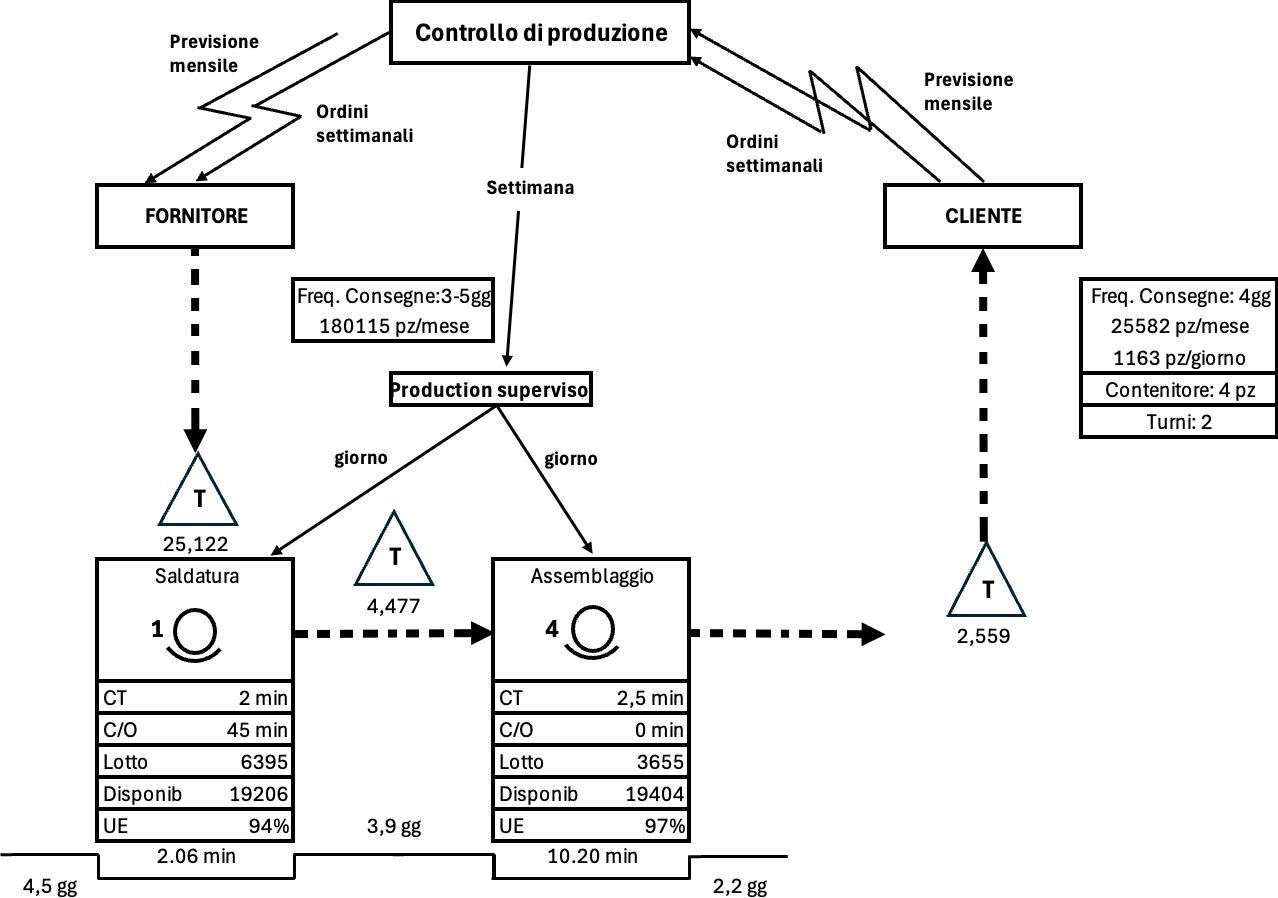
\includegraphics[width=\textwidth]{images/Value Stream Map A1.png}
    \caption{Value Stream Map A1}
    \label{fig: Value Stream Map A1}
\end{figure}

\noindent
Per consultare le VSM complete per tutti i prodotti, è possibile fare riferimento all'allegato "{{excelCompleto}}".
\newpage

\subsection{Valutazione ottimizzazioni processo produttivo}
\subsubsection{Ottimizzazione dell'OEE}
Per le ottimizzazioni che riguardano l'OEE si è cercato di agire sulle ore in una giornata, cioè la durata di un turno, oppure sul numero di giorni di lavoro in un mese.\\
Cambiando le ore in giorno di lavoro da \(15\) ore a \(14,\bar{3}\) ore, equivalenti a turni da 7 ore e 10 minuti, si riesce a migliorare l'OEE di circa il \(3,5\%\) per l'assemblaggio, mentre la saldatura perde il \(5\%\), rimanendo comunque con un OEE del \(81,65\%\).\\
La variazione delle ore è contenuta per non variare eccessivamente il numero di box di saldatura, il numero di linee di assemblaggio e il numero di carrelli elevatori, il cui aumento sarebbe conseguenza di una finestra di tempo ridotta per gestire le merci in arrivo e in consegna.\\
Se gli elementi sopra variassero troppo significativamente, il vantaggio derivante dal miglioramento dell'OEE sarebbe nullificato dai costi legati ad un maggior numero di dipendenti e attrezzature.\\
Inoltre si è notato che l'OEE e la saturazione del reparto di saldatura aumenta significativamente (\(+7\%\)) unificando tutte le categorie di prodotti in unico reparto anziché tenendoli separati in A1-B e A2-D; questo è giustificato dal fatto che il numero di postazioni teoriche (\(N_{\text{th}}\)), senza mettere insieme i due reparti, è più lontano dal numero arrotondato dopo averli messi insieme.
\newpage

\subsection{Calcolo EPEI}
Per determinare l'EPEI si è scelto di mettere in comune le linee di assemblaggio di A1-A2 e B-D poiché formate dallo stesso numero di postazioni, in questo modo nessuna delle postazioni sarebbe mai inutilizzata.\\
Per il reparto di saldatura sono stati messi in comune tutti i box, come citato sopra.\\

\noindent
Per il calcolo dell'EPEI si procede come segue:
\begin{align}
    & D_m = \frac{D}{N} \\
    & L = \frac{D_m}{g} \\
    & T_\text{run} = \text{TC} \times L \\
    & T_\text{tot} = T_\text{set} + T_\text{run} \\
    & \text{EPEI} = \frac{T_s}{T_p - T_\text{tot}} \\
    & L_\text{EPEI} = \text{EPEI} \times d
\end{align}

\vspace{1em}
\noindent
dove le grandezze sono:
\begin{itemize}
    \item $D$: domanda complessiva mensile
    \item $N$: numero di postazioni produttive
    \item $D_m$: domanda mensile per postazione
    \item $g$: giorni lavorativi mensili
    \item $L$: lotto di produzione giornaliero
    \item $T_\text{set}$: tempo di setup
    \item $T_\text{run}$: tempo totale di produzione del lotto
    \item $T_\text{tot}$: tempo totale necessario per completare il setup e la produzione del lotto
    \item $T_p$: tempo produttivo disponibile in un turno
    \item $d$: domanda giornaliera complessiva
    \item $L_{\text{EPEI}}$: lotto calcolato in base all'EPEI
\end{itemize}
\newpage


\section{Valutazione dell'investimento}
\begin{table}[h!]
    \centering
    \resizebox{\textwidth}{!}{
    \renewcommand{\arraystretch}{1.5}
    \begin{tabular}{|l|c|r|r|r|}
        \hline
        \textbf{Item} & \textbf{UN.} & \textbf{Importo unitario} & \textbf{\#/dimensione} & \textbf{Importo totale} \\
        \hline
        Box saldatura & €/cad & 30\,000 & 11 & 330\,000\,€ \\
        Linea di montaggio & €/m & 6\,000 & 154 & 924\,000\,€ \\
        Edificio industriale & €/m\textsuperscript{2} & 1\,000 & 19\,132 & 19\,132\,000\,€ \\
        Impianti generali & €/m\textsuperscript{2} & 410 & 19\,132 & 7\,844\,120\,€ \\
        Scaffalature tradizionali & €/cad & 100 & 240 & 24\,000\,€ \\
        Scaffalature drive-through & €/cad & 80 & 13\,140 & 1\,051\,200\,€ \\
        Carrelli elevatori & €/cad & 30\,000 & 68 & 2\,040\,000\,€ \\
        Trenini & €/cad & 30\,000 & 2 & 60\,000\,€ \\
        Trasportatori a rulli folli & €/m & 600 & 160.2 & 96\,120\,€ \\
        Trasportatori a rulli motorizzati & €/m & 2\,500 & 86.9 & 217\,250\,€ \\
        Portoni & €/cad & 9\,700 & 13 & 126\,100\,€ \\
        Bocche di carico & €/cad & 3\,500 & 8 & 28\,000\,€ \\
        Trituratore & €/cad & 75\,000 & 1 & 75\,000\,€ \\
        Porte di sicurezza & €/cad & 2\,800 & 13 & 36\,400\,€ \\
        Terreno & € & 600\,000 & 1 & 600\,000\,€ \\
        \hline
        \textbf{Totale} & & & & \textbf{32\,584\,090\,€} \\
        \hline
    \end{tabular}
    }
    \caption{Riepilogo costi per item}
\end{table}
\newpage


\section{Allegati}
Per facilitare la consultazione, sono stati inseriti gli allegati in cui sono riportati i calcoli e le tabelle utilizzate per la realizzazione del progetto.
\vskip1em
Per la loro visualizzazione, è possibile \underline{\textbf{cliccare l'icona corrispondente}} e, a seconda della tipologia di allegato, verrà aperto il file su Excel, AutoCAD o direttamente su Adobe Acrobat Reader.
\begin{table}[h!]
    \centering
    \captionsetup{justification=centering}
    \resizebox{0.7\textwidth}{!}{
    \renewcommand{\arraystretch}{1.5}
    \begin{tabular}{|l|c|}
        \hline
        \textbf{Allegato} & \textbf{Software} \\
        \hline
        {{excelA1B}} & Excel \\
        {{excelA2D}} & Excel \\
        {{matriceWBSOBS}} & Excel \\
        {{excelCompleto}} & Excel \\
        {{gantt}} & Excel \\
        {{ariaCompressaAssemblaggio}} & Excel \\
        {{distintaBase}} & PDF \\
        {{processoProduttivo}} & PDF \\
        {{elevatoreBTSTAXIO}} & PDF \\
        {{transpalletBTLIFTER}} & PDF \\
        {{layoutPostazioneSaldatura}} & PDF \\
        {{layoutPostazioneAssemblaggio}} & PDF \\
        {{areaRicezione}} & PDF \\
        {{areaPicking}} & PDF \\
        {{areaInterna}} & PDF \\
        {{areaRicarica}} & PDF \\
        {{areaParcheggi}} & PDF \\
        {{collocazioneStabilimento}} & PDF \\
        {{spaghettiChartA1}} & PDF \\
        {{spaghettiChartB}} & PDF \\
        {{spaghettiChartA2}} & PDF \\
        {{spaghettiChartD}} & PDF \\
        {{planimetriaInternoEsterno}} & PDF \\
        {{planimetriaInternaConPiani}} & PDF \\
        \hline
    \end{tabular}
    }
    \caption{Riepilogo allegati}
\end{table}


\newpage
\printbibliography
\end{document}
